%%
%% This is file `sample-sigplan.tex',
%% generated with the docstrip utility.
%%
%% The original source files were:
%%
%% samples.dtx  (with options: `sigplan')
%% 
%% IMPORTANT NOTICE:
%% 
%% For the copyright see the source file.
%% 
%% Any modified versions of this file must be renamed
%% with new filenames distinct from sample-sigplan.tex.
%% 
%% For distribution of the original source see the terms
%% for copying and modification in the file samples.dtx.
%% 
%% This generated file may be distributed as long as the
%% original source files, as listed above, are part of the
%% same distribution. (The sources need not necessarily be
%% in the same archive or directory.)
%%
%% Commands for TeXCount
%TC:macro \cite [option:text,text]
%TC:macro \citep [option:text,text]
%TC:macro \citet [option:text,text]
%TC:envir table 0 1
%TC:envir table* 0 1
%TC:envir tabular [ignore] word
%TC:envir displaymath 0 word
%TC:envir math 0 word
%TC:envir comment 0 0
%%
%%
%% The first command in your LaTeX source must be the \documentclass command.
% \documentclass[sigplan,screen]{acmart}

\documentclass[sigplan,10pt]{acmart}
\renewcommand\footnotetextcopyrightpermission[1]{}

\usepackage{listings}
\usepackage{tikz}
\usepackage{amsthm}
\usepackage{graphicx}
\usepackage{subcaption}
\usepackage{algorithm}
%\usepackage{algorithmic}
\usepackage{algpseudocode}
\usepackage{tabularx,booktabs}
\usepackage{multirow}

\newcommand{\CommentOut}[1]{}
\newcommand\TODO[1]{\textcolor{red}{TODO #1}}
\newcommand\COMMENT[1]{\textcolor{green}{COMMENT #1}}
\newcommand{\Treebeard}{{\sc {SilvanForge}}}
\newcommand{\TreebeardOLD}{{\sc {Treebeard}}}
\newcommand{\op}[1]{{\texttt {#1}}}

\definecolor{codegreen}{rgb}{0,0.6,0}
\definecolor{codegray}{rgb}{0.5,0.5,0.5}
\definecolor{codepurple}{rgb}{0.58,0,0.82}
% \definecolor{backcolour}{rgb}{0.95,0.95,0.92}
\definecolor{backcolour}{HTML}{F2F7FC}
\definecolor{circlegreen}{rgb}{0.44,0.78,0.28}
\definecolor{circleblue}{rgb}{0.27,0.45,0.77}
\definecolor{circleorange}{HTML}{F4B183}
\definecolor{MidnightBlue}{HTML}{006795}
\definecolor{OliveGreen}{HTML}{3C8031}
\definecolor{OrangeCircleOutline}{HTML}{C55A11}

\newcommand*\circled[1]{\tikz[baseline=(char.base)]{
            \node[shape=circle, draw=OliveGreen, inner sep=1pt, fill=circlegreen, text=white] (char) {#1};}}
\newcommand*\bluecircled[1]{\tikz[baseline=(char.base)]{
            \node[shape=circle, draw=MidnightBlue, inner sep=1pt, fill=circleblue, text=white] (char) {#1};}}
\newcommand*\orangecircled[1]{\tikz[baseline=(char.base)]{
              \node[shape=circle, draw=OrangeCircleOutline, inner sep=1pt, fill=circleorange, text=white] (char) {#1};}}

\lstdefinestyle{c++}{language=C++,
    morekeywords={ensemble, getTree, getRoot, isLeaf, isLeafTile, traverseTreeTile, getLeafValue, loadThresholds,
                  loadFeatureIndices, loadTileShape, getChildTile, parallel, par, InterleavedWalk, evaluateTilePredicates,
                  getChildTile, WalkDecisionTree, walkDecisionTree, moveToChildTile, to, step, tile, split, unroll,
                  reorder, specialize, unrollDepth, unrollWalk, reduce, gpuDimension},
    backgroundcolor=\color{backcolour},
    commentstyle=\color{codegreen},
    keywordstyle=\color{blue},
    numberstyle=\tiny\color{codegray},
    stringstyle=\color{codepurple},
    basicstyle=\scriptsize,
    breakatwhitespace=false,
    breaklines=true,
    captionpos=b,
    keepspaces=true,
    numbers=left,
    numbersep=5pt,
    showspaces=false,
    showstringspaces=false,
    showtabs=false,
    tabsize=2
}

\lstset{style=c++}


%% NOTE that a single column version is required for 
%% submission and peer review. This can be done by changing
%% the \doucmentclass[...]{acmart} in this template to 
%% \documentclass[manuscript,screen,review]{acmart}
%% 
%% To ensure 100% compatibility, please check the white list of
%% approved LaTeX packages to be used with the Master Article Template at
%% https://www.acm.org/publications/taps/whitelist-of-latex-packages 
%% before creating your document. The white list page provides 
%% information on how to submit additional LaTeX packages for 
%% review and adoption.
%% Fonts used in the template cannot be substituted; margin 
%% adjustments are not allowed.
%%
%% \BibTeX command to typeset BibTeX logo in the docs
\AtBeginDocument{%
  \providecommand\BibTeX{{%
    \normalfont B\kern-0.5em{\scshape i\kern-0.25em b}\kern-0.8em\TeX}}}

%% Rights management information.  This information is sent to you
%% when you complete the rights form.  These commands have SAMPLE
%% values in them; it is your responsibility as an author to replace
%% the commands and values with those provided to you when you
%% complete the rights form.
% \setcopyright{acmlicensed}
% \copyrightyear{2018}
% \acmYear{2018}
% \acmDOI{XXXXXXX.XXXXXXX}

%% These commands are for a PROCEEDINGS abstract or paper.
% \acmConference[Conference acronym 'XX]{Make sure to enter the correct
%   conference title from your rights confirmation emai}{June 03--05,
%   2018}{Woodstock, NY}
%
%  Uncomment \acmBooktitle if th title of the proceedings is different
%  from ``Proceedings of ...''!
%
%\acmBooktitle{Woodstock '18: ACM Symposium on Neural Gaze Detection,
%  June 03--05, 2018, Woodstock, NY} 
%\acmISBN{978-1-4503-XXXX-X/18/06}


%%
%% Submission ID.
%% Use this when submitting an article to a sponsored event. You'll
%% receive a unique submission ID from the organizers
%% of the event, and this ID should be used as the parameter to this command.
%%\acmSubmissionID{123-A56-BU3}

%%
%% For managing citations, it is recommended to use bibliography
%% files in BibTeX format.
%%
%% You can then either use BibTeX with the ACM-Reference-Format style,
%% or BibLaTeX with the acmnumeric or acmauthoryear sytles, that include
%% support for advanced citation of software artefact from the
%% biblatex-software package, also separately available on CTAN.
%%
%% Look at the sample-*-biblatex.tex files for templates showcasing
%% the biblatex styles.
%%

%%
%% The majority of ACM publications use numbered citations and
%% references.  The command \citestyle{authoryear} switches to the
%% "author year" style.
%%
%% If you are preparing content for an event
%% sponsored by ACM SIGGRAPH, you must use the "author year" style of
%% citations and references.
%% Uncommenting
%% the next command will enable that style.
%%\citestyle{acmauthoryear}

%%
%% end of the preamble, start of the body of the document source.
\begin{document}

%%
%% The "title" command has an optional parameter,
%% allowing the author to define a "short title" to be used in page headers.
\title{{\textbf{\Treebeard{}}} : A Schedule Guided Retargetable Compiler for Decision Tree Inference}

%%
%% The "author" command and its associated commands are used to define
%% the authors and their affiliations.
%% Of note is the shared affiliation of the first two authors, and the
%% "authornote" and "authornotemark" commands
%% used to denote shared contribution to the research.

% \author{Ben Trovato}
% \authornote{Both authors contributed equally to this research.}
% \email{trovato@corporation.com}
% \orcid{1234-5678-9012}
% \author{G.K.M. Tobin}
% \authornotemark[1]
% \email{webmaster@marysville-ohio.com}
% \affiliation{%
%   \institution{Institute for Clarity in Documentation}
%   \streetaddress{P.O. Box 1212}
%   \city{Dublin}
%   \state{Ohio}
%   \country{USA}
%   \postcode{43017-6221}
% }

% \author{Lars Th{\o}rv{\"a}ld}
% \affiliation{%
%   \institution{The Th{\o}rv{\"a}ld Group}
%   \streetaddress{1 Th{\o}rv{\"a}ld Circle}
%   \city{Hekla}
%   \country{Iceland}}
% \email{larst@affiliation.org}

% \author{Valerie B\'eranger}
% \affiliation{%
%   \institution{Inria Paris-Rocquencourt}
%   \city{Rocquencourt}
%   \country{France}
% }

% \author{Aparna Patel}
% \affiliation{%
%  \institution{Rajiv Gandhi University}
%  \streetaddress{Rono-Hills}
%  \city{Doimukh}
%  \state{Arunachal Pradesh}
%  \country{India}}

% \author{Huifen Chan}
% \affiliation{%
%   \institution{Tsinghua University}
%   \streetaddress{30 Shuangqing Rd}
%   \city{Haidian Qu}
%   \state{Beijing Shi}
%   \country{China}}

% \author{Charles Palmer}
% \affiliation{%
%   \institution{Palmer Research Laboratories}
%   \streetaddress{8600 Datapoint Drive}
%   \city{San Antonio}
%   \state{Texas}
%   \country{USA}
%   \postcode{78229}}
% \email{cpalmer@prl.com}

% \author{John Smith}
% \affiliation{%
%   \institution{The Th{\o}rv{\"a}ld Group}
%   \streetaddress{1 Th{\o}rv{\"a}ld Circle}
%   \city{Hekla}
%   \country{Iceland}}
% \email{jsmith@affiliation.org}

% \author{Julius P. Kumquat}
% \affiliation{%
%   \institution{The Kumquat Consortium}
%   \city{New York}
%   \country{USA}}
% \email{jpkumquat@consortium.net}

%%
%% By default, the full list of authors will be used in the page
%% headers. Often, this list is too long, and will overlap
%% other information printed in the page headers. This command allows
%% the author to define a more concise list
%% of authors' names for this purpose.
% \renewcommand{\shortauthors}{Trovato and Tobin, et al.}

%%
%% The abstract is a short summary of the work to be presented in the
%% article.
% \begin{abstract}
%   A clear and well-documented \LaTeX\ document is presented as an
%   article formatted for publication by ACM in a conference proceedings
%   or journal publication. Based on the ``acmart'' document class, this
%   article presents and explains many of the common variations, as well
%   as many of the formatting elements an author may use in the
%   preparation of the documentation of their work.
% \end{abstract}

%%
%% The code below is generated by the tool at http://dl.acm.org/ccs.cfm.
%% Please copy and paste the code instead of the example below.
%%
\begin{CCSXML}
% <ccs2012>
%  <concept>
%   <concept_id>00000000.0000000.0000000</concept_id>
%   <concept_desc>Do Not Use This Code, Generate the Correct Terms for Your Paper</concept_desc>
%   <concept_significance>500</concept_significance>
%  </concept>
%  <concept>
%   <concept_id>00000000.00000000.00000000</concept_id>
%   <concept_desc>Do Not Use This Code, Generate the Correct Terms for Your Paper</concept_desc>
%   <concept_significance>300</concept_significance>
%  </concept>
%  <concept>
%   <concept_id>00000000.00000000.00000000</concept_id>
%   <concept_desc>Do Not Use This Code, Generate the Correct Terms for Your Paper</concept_desc>
%   <concept_significance>100</concept_significance>
%  </concept>
%  <concept>
%   <concept_id>00000000.00000000.00000000</concept_id>
%   <concept_desc>Do Not Use This Code, Generate the Correct Terms for Your Paper</concept_desc>
%   <concept_significance>100</concept_significance>
%  </concept>
% </ccs2012>
\end{CCSXML}

% \ccsdesc[500]{Do Not Use This Code~Generate the Correct Terms for Your Paper}
% \ccsdesc[300]{Do Not Use This Code~Generate the Correct Terms for Your Paper}
% \ccsdesc{Do Not Use This Code~Generate the Correct Terms for Your Paper}
% \ccsdesc[100]{Do Not Use This Code~Generate the Correct Terms for Your Paper}

%%
%% Keywords. The author(s) should pick words that accurately describe
%% the work being presented. Separate the keywords with commas.
\keywords{}

%% A "teaser" image appears between the author and affiliation
%% information and the body of the document, and typically spans the
%% page.
% \begin{teaserfigure}
%   \includegraphics[width=\textwidth]{sampleteaser}
%   \caption{Seattle Mariners at Spring Training, 2010.}
%   \Description{Enjoying the baseball game from the third-base
%   seats. Ichiro Suzuki preparing to bat.}
%   \label{fig:teaser}
% \end{teaserfigure}

% \received{20 February 2007}
% \received[revised]{12 March 2009}
% \received[accepted]{5 June 2009}

%%
%% This command processes the author and affiliation and title
%% information and builds the first part of the formatted document.

\begin{comment}
\begin{abstract}
  Decision tree based models are generated by some of the most commonly 
  used machine learning algorithms like gradient boosting and random forests.
  These algorithms are used very widely in practice and the resulting models
  are deployed to production at scale. The models are served on a variety of 
  machines including CPUs and GPUs and inference performance on all these 
  machines is an important consideration. On CPUs, models are served using
  either libraries such as XGBoost, Sklearn, and LightGBM or specialized 
  compilers like \TreebeardOLD{}, Treelite, and Hummingbird. On GPUs, XGBoost 
  and RAPIDs FIL are popular libraries. However, these libraries and compilers
  do not provide portable performance across the targets of interest. They 
  also leave significant optimization opportunities unexplored. 

  In this paper, we present the design of \Treebeard{}, a compiler infrastructure 
  for decision tree based models that significantly expands the design space 
  that can be explored and provides portable performance across CPU and GPU 
  targets. We rearchitect the open-source \Treebeard{} infrastructure 
  and significantly extend it to enable high-performance code generation 
  across target processors. Specifically, we design a scheduling language 
  that encapsulates the large optimization space for decision tree inference
  and develop techniques to explore this space. Further,
  we design techniques to represent and optimize parallel reductions, extend
  \TreebeardOLD{}'s intermediate representations to include operations like caching
  and rearchitect \TreebeardOLD{} to allow in-memory representations to be built 
  as plugins. \TODO{Need to say we investigate how to structure a compiler for 
  decision tree inference that can target multiple hardware platforms}

  We implement \Treebeard{} using the MLIR compiler infrastructure and
  compare the performance of the generated code against state-of-the-art
  systems on CPUs and GPUs. On GPUs we compare performance against XGBoost,
  RAPIDs FIL, and Tahoe. We find that \Treebeard{} is significantly faster
  than other systems that target GPUs across a wide range of batch sizes 
  and models on different NVIDIA GPUs. \Treebeard{} is an order of magnitude faster than XGBoost and
  about 2-3$\times$ faster than RAPIDs FIL and Tahoe on average. \TODO{Make 
  this more precise. But how?}. We also show how \Treebeard{} can generate  
  high-performance code on other GPUs by running the benchmarks on an AMD GPU.
  On CPUs, we compare against \TreebeardOLD{} and show how the  
  optimization opportunities exposed by \Treebeard{}'s scheduling 
  language allow it to generate higher performance code by specializing  
  code for different batch sizes.
\end{abstract}
\end{comment}
\begin{abstract}
  
  With the rapid proliferation of machine learning, the demand for on-device model inference has surged. Concurrently, the hardware ecosystem is evolving rapidly, leading to an increasing heterogeneity in client machines.
  %While CPUs have been the mainstay for machine learning inference, the availability of GPUs holds promise to scale to bigger and more powerful models. 
  This paper is motivated by the problems encountered when targeting inference of decision tree based models, the most popular models on tabular data, to run at peak performance on diverse client hardware. We evaluated existing solutions and found that they do not provide portable performance across different hardware targets.
  %Decision tree based models are widely used in practice due to their robustness, interpretability, and ability to handle missing data.  
  
  To address this we present the design of \Treebeard{}, a schedule guided compiler infrastructure 
  for decision tree based models that searches over a large design space 
  to find high performance schedules on a diverse set of CPU and GPU 
  targets. 
  %We re-architect the open-source \TreebeardOLD{} infrastructure and significantly extend it to enable high-performance code generation across target processors. 
  \Treebeard{} has two core components. A scheduling language 
  that encapsulates the large optimization space for decision tree inference, 
  and techniques to efficiently explore this space.
  \TODO{include some keywords from the language and space complexity}.
  %We also design a set of heuristics that can find near-optimal solutions in quick time.
  Second, an optimizing multi-level compiler that can generate code based on the schedule. 
  For the latter, we re-architect the open-source \TreebeardOLD{} CPU compiler to support schedule guided compilation and
add support for GPU code generation. We further enhance the compiler with fundamental new optimization interfaces for caching, parallel reduction, and a plug-in mechanism to explore different in-memory representations of trees.
  
  %The compiler builds on an existing compiler for CPUs, \TreebeardOLD{}, also add support for caching, parallel reduction and a plug-in mechanism to explore different in-memory representations of trees.

  We evaluate \Treebeard{} on \TODO{kr:Can we quote a number} a large number of diverse models and demonstrate that the best schedule varies drastically with model, batch size, and target hardware. 
  Despite this, the scheduling heuristic is able to quickly find near optimal schedules while searching over a small fraction of the total search space.
  In terms of performance, \Treebeard{} generated code  
   is an order of magnitude faster than XGBoost and
  about 2-3$\times$ faster on average than RAPIDs FIL and Tahoe. \TODO{Make 
  this more precise. But how?}. While these systems only generate code for Nvidia, \Treebeard{} achieves competent performance on AMD GPUs as well. 
  On CPUs, we compare against \TreebeardOLD{} and show how the  
  optimization opportunities exposed by \Treebeard{}'s scheduling 
  language allow it to generate higher performance code by specializing  
  code for different batch sizes.
  \TODO{(numbers for CPU performance?)}
\end{abstract}

\maketitle
\section{Introduction}
\label{sec:intro}
We are in the midst of a hardware revolution, a new golden age for computer architecture~\cite{GoldenAge}. The last 
decade has seen a shift in architectural paradigms, with the rise of GPUs and accelerators. This shift has been driven
by the necessity to innovate in the post Moore's law and Dennard's scaling era. This transformation has also played 
a significant role in the success of modern deep learning models, as they enable scaling model training and inference 
to a massive number of threads. Such scalability would be essential for all performance critical applications, including
other machine learning models that need to scale with increasing data sizes and model complexities. 
%need to accelerate machine learning workloads. The success of modern AI models is due to their ability to scale both training and inference to a massive number of threads. This has been made possible by the rise of GPUs and accelerators.

%Despite these recent advancements, one dominant family of models, namely decision forest models have not seen the same level of acceleration.
Decision forest models remain the mainstay for machine learning over tabular data~\cite{DLNotAllYouNeed,TreebasedOutperformDL}. 
Their robustness, interpretability, and ability to handle missing data make them a popular choice for a wide range of applications. 
\TODO{a few more lines, classification, regression, etc.}
%We observe that while scalable performance on neural network models has received significant attention, decision tree inference has not seen the same level of acceleration.
A recent survey~\cite{kaggle}\dots. 
The survey also finds that, the cost of inference is the most critical factor in the overall cost of deploying a machine learning model.
This is because, in production settings, each model is trained once and often used for inference a few thousand times. 
%

This paper is motivated by the need to accelerate decision tree inference to achieve portable performance on a variety of client hardware.
In particular, we focus on portable performance across a range of commodity CPUs and low-to-mid-range GPUs, a class of hardware that has seen widespread adoption across client/edge devices used for inference.

Decision forest models are composed of a large collection of decision trees (100-1000), and inference involves traversing down each tree in the forest and aggregating the predictions. Inference is typically done in a batched setting, where multiple inputs are processed simultaneously.

%Despite the simplicity of the model, decision tree inference is computationally expensive, and is surprisingly hard to scale to a large number of threads
Despite the simplicity of the model and the availability of multiple sources of coarse grain parallelism (parallelism across inputs in a batch and parallelism across trees), existing systems do not consistently scale well across different models. 
This is because existing systems exploit a limited set of optimizations and often specialize the implementation to a specific hardware platform, which limits their portability. 

%\TODO{cover Rapids, Tahoe, XGBoost and Treebeard}.  
Evaluation on a diverse set of models highlights that the best implementation often requires a careful combination of many optimization strategies. For example, managing the working set of nodes across a set of trees is critical to get scalable performance. This requires a combination of techniques like data layout optimizations, loop transformations, and memory access optimizations. Existing systems each use specific data layouts for the underlying tree (XGBoost uses a sparse representation, RAPIDs FIL uses what is called the reorg representation 
and Tahoe uses a variation of the reorg representation) and propose simple loop transformations (XGBoost uses \dots()) that together determine the accesses patterns and the working set. They do not perform consistently well across different models and hardware platforms.
Managing the working set is just one of several optimizations that are critical for high-performance decision tree inference.
 \TODO{Improve the next line}
 Others include tree ordering,  incremental reduction of predicted values, interleaving across multiple trees, and so on.

This paper presents \Treebeard{}, a novel schedule guided compilation infrastructure for decision tree inference on multiple target hardware. \Treebeard{} is able to generate high-performance code for decision tree inference by exploring a large optimization space. The code generation is guided by a \emph{schedule} object that allows us to effectively represent this solution space abstractly. The schedule object is written in \Treebeard{} custom scheduling language that is expressive enough to represent a wide range of implementation strategies. We demonstrate that the language is sufficient to express the various optimizations proposed by prior work, and further generalizes them and incorporates several new optimizations. We also design and implement a heuristic that is able to quickly find high-performance schedules for the model being compiled.
\TODO{Performance evaluation summary}
\TODO{Oganization}
\subsection{Contributions}
\begin{itemize}
  \item We present the design for a multi-target decision tree compiler infrastructure and implement several optimizations within this framework.
   We are also the first to implement an optimizing compiler for decision tree inference on GPUs.
  \item We identify that an extensive optimization space exists for the problem of decision tree inference. We design a scheduling language that 
  allows us to effectively represent this solution space abstractly. This scheduling language is expressive enough to represent a wide range of  
  implementation strategies proposed by prior work.
  \item To the best of our knowledge, we perform the first extensive characterization of the optimization space for decision tree inference 
  on GPUs. Using some of the characteristics we identify, we design and implement a heuristic that is able to quickly find high-performance 
  schedules for the model being compiled. 
  \item We design and implement a general framework for expressing and optimizing reductions within MLIR. To the best of our knowledge, this is the first
  such framework.
  \item We evaluate our implementation by comparing it against RAPIDs and Tahoe, the state-of-the-art decision tree inference frameworks for GPU and 
  report significant speedups. We also show that our compiler can effectively target different GPUs, including both NVIDIA and AMD GPUs.
\end{itemize}
\section{Motivation}

In this section, we first motivate the need for a scheduling language 
by showing how a model can be compiled in different ways using the example
in Figure \ref{Fig:HIRExample} and subsequently, we show how drastically 
performance can vary across these variants for real benchmarks.

First, we consider the schedule that processes one tree at a time 
for all input rows and unrolls all tree walks. 
The schedule splits the loop over the trees into two loops -- one that
iterates over the first two trees (Trees 1 and 2 with depth 1) and 
the second that iterates over the last two trees (Trees 3 and 4 with
depth 2). The schedule then unrolls the tree walks for each tree.
\begin{lstlisting}[style=c++]
  reorder(tree, batch)  
  split(tree, t0, t1, 2)
  unrollWalk(t0, 1)
  unrollWalk(t1, 2)
\end{lstlisting}
The concrete implementation of this schedule (in one of \Treebeard{}'s IRs) 
is as follows.
\begin{lstlisting}[style=c++]
  model = ensemble(...)
  for t0 = 0 to 2 step 1 {
    T = getTree(ensemble, t0)
    for batch = 0 to BATCH_SIZE step 1 {
      treePred = walkDecisionTree(T, 
                    input[batch]) <unrollDepth = 1>
      reduce(result[batch], treePred)
    }
  }
  for t1 = 2 to 4 step 1 {
    T = getTree(ensemble, t0)
    for batch = 0 to BATCH_SIZE step 1 {
      treePred = walkDecisionTree(T,
                    input[batch]) <unrollDepth = 2>
      reduce(result[batch], treePred) <'+', 0.0>
    }
  }
\end{lstlisting}
This schedule is ideally suited for a single-core CPU. It maximizes 
the reuse of trees in the L1 cache and also minimizes the amount of
branching by unrolling tree walks. However, it doesn't exploit  
any parallelism and is therefore ill-suited for parallel processors.

One form of parallelism that can be exploited is to process rows in 
parallel. However, with massively parallel processors like GPUs,
this may not yield sufficient parallel work. Another option is to also 
parallelize across trees. A possible schedule to accomplish this is as follows.
\begin{lstlisting}[style=c++]
  tile(tree, t0, t1, 2)
  reorder(batch, t1, t0)
  split(t0, t0_1, t0_2, 2)
  unrollWalk(t0_1, 1)
  unrollWalk(t0_2, 2)
  gpuDimension(batch, grid.x)
  gpuDimension(t1, block.x)
\end{lstlisting}
This schedule generates an inference function that runs on the GPU. 
The inference routine processes one input row per thread block (since the \op{batch}
loop is mapped directly to \op{grid.x}).
It also splits the trees into two sets by tiling the \op{tree} loop.
Each of the two sets is processed in parallel. We unroll the tree walks 
for each tree. The IR generated is as follows. 
\begin{lstlisting}[style=c++]
  model = ensemble(...)
  par.for batch = 0 to BATCH_SIZE step 1 <grid.x> {
    par.for t1 = 0 to 2 step 1 <block.x> {
      for t0_1 = 0 to 2 step 2 {
        T = getTree(ensemble, t0_1 + t1)
        treePred = walkDecisionTree(T, 
                        input[batch]) <unrollDepth = 1>
        reduce(result[batch], treePred)
      }
      for t0_2 = 2 to 4 step 2 {
        T = getTree(ensemble, t0_2 + t1)
        treePred = walkDecisionTree(T,
                        input[batch]) <unrollDepth = 2>
        reduce(result[batch], treePred) <'+', 0.0>
      }
    }
  }
\end{lstlisting}

In the case of this schedule, the \op{reduce}
operation needs special consideration. In order to correctly generate 
code for this schedule, the compiler needs to determine that parallel 
iterations of the \op{t1} 
loop accumulate into the same element of the \op{result} array.
One possible solution is to rewrite the reduction so that each parallel 
iteration accumulates into a different array element by introducing 
a temporary buffer (\op{tempResults}) as follows.
\begin{lstlisting}[style=c++]
  float tempResults[2][BATCH_SIZE]
  model = ensemble(...)
  par.for batch = 0 to BATCH_SIZE step 1 <grid.x> {
    par.for t1 = 0 to 2 step 1 <block.x> {
      for t0_1 = 0 to 2 step 2 {
        T = getTree(ensemble, t0_1 + t1)
        treePred = walkDecisionTree(T, 
                      input[batch]) <unrollDepth = 1>
        reduce(tempResults[t1][batch], treePred)
      }
      for t0_2 = 2 to 4 step 2 {
        T = getTree(ensemble, t0_2 + t1)
        treePred = walkDecisionTree(T,
                      input[batch]) <unrollDepth = 2>
        reduce(tempResults[t1][batch], treePred) <'+', 0.0>
      }
    }
    result[batch] = reduce_dimension(tempResults[:][batch], 0)
  }
\end{lstlisting}
Here, partial results are accumulated into \op{tempResults} and then
reduced across the \op{t1} dimension (represented by the \op{reduce\_dimension}
operation) to get the final result.

As is evident from these examples, it is possible to optimize 
the inference routine in different ways. Also, the structure of the loop 
nest in the inference routine can get quite complex even 
for simple schedules. Writing these routines by hand 
is error-prone and time-consuming.  We believe that designing a 
scheduling language to encapsulate these strategies and a principled code 
generator to automatically generate code based on the schedule is the 
best approach. 

We find that these different strategies can have significantly different
performance. Figure \ref{fig:sensitivity} shows the\dots.

Several problems need to be solved in order to build the kind of 
schedule guided retargetable compiler required. We had to enable the
compiler to represent and optimize reductions, deal uniformly with different
in-memory representations of the model, design optimizations to effectively 
use the memory hierarchy of the target processor (shared memory on GPUs and 
cache on the CPU) and finally be able to generate target specific code. 
The rest of the paper describes these challenges in detail and how we
solved them in \Treebeard{}.

% Our main aim while designing \Treebeard{} was to unify the diverse set of implementation
% strategies that have been used in existing systems for decision tree inference. Some 
% differences in these systems are as follows:
% \begin{itemize}
%   \item Decision tree inference is run on several platforms including CPUs and GPUs. The 
%   implementations used on each of these platforms are different and the techniques used
%   to optimize them are also different.
%   \item A diverse set techniques have been proposed for optimization of decision tree 
%   inference on CPUs and GPUs \cite{VPred, Tahoe, Treelite, XGBoost, Hummingbird, QuickScorer, FIL}. 
%   No system exists that unifies the disparate optimizations implemented in these systems.
%   \item A very extensive design space of optimizations exists for decision tree inference
%   outside the few that have been proposed in the literature. However, currently no 
%   system exists that is capable of exploring this space and identifying the best set 
%   of parameters to use for a given model and platform.
%   \item Different systems use different in-memory representations for the model. For example,
%   XGBoost uses a sparse representation, RAPIDs FIL uses what is called the reorg representation 
%   and Tahoe uses a variation of the reorg representation. Currently, systems implement 
%   inference kernels that are tied to a single representation of the model. Again, this means
%   that no current system can explore different combinations of in-memory representations 
%   and optimizations.
% \end{itemize}
% At high-level, to make \Treebeard{} capable of unifying these differences, we design 1)  
% expressive intermediate representations that can represent and compose several proposed 
% optimizations 2) a scheduling language that specifies the structure of the
% generated code and 3) a plugin mechanism with which different in-memory representations
% can be composed with different optimizations. Finally, we develop a heuristic to
% explore the extensive optimization space that \Treebeard{}'s design enables.

% While a diverse set techniques have been proposed for optimization of decision tree 
% inference on CPUs and GPUs \cite{VPred, Tahoe, Treelite, XGBoost, Hummingbird, QuickScorer, FIL},
% a very extensive design space of optimizations exists 
% outside what has been proposed in the literature. Furthermore, decision tree inference 
% is run on several platforms including CPUs and GPUs. The implementations used on each of 
% these platforms are different and the techniques used to optimize them are different.
% To make matters even more complicated, several in-memory representations
% have been proposed for decision tree models. For example, XGBoost\cite{XGBoost} uses a sparse representation,
% RAPIDs FIL\cite{FIL} uses what is called the reorg representation and Tahoe uses a variation of the reorg
% representation. 
% \TODO{Can we add some numbers here to show that different models/batch sizes need different optimizations?}

% To solve the problems of exploring the design space of optimizations for decision tree
% inference and enabling portable performance, we build several techniques in \Treebeard{}, 
% an open source compiler infrastructure for decision tree inference. To make \Treebeard{}
% capable of unifying these different techniques and targets, we do the following. 
% \begin{itemize}
%   \item We design a scheduling language that encapsulates various optimization techniques
%   and controls the structure of the generated code.
%   \item We design an MLIR dialect to represent and optimize reductions and use this 
%   dialect within \Treebeard{} to enable the generation of different variants of 
%   inference routines.
%   \item We extend \Treebeard{}'s intermediate representations to include operations like caching.
%   We were able to easily reuse and extend \Treebeard{}'s IR as it was built as an MLIR dialect.
%   \item We design a plugin mechanism with which different in-memory representations
%   can be composed with different optimizations.  
% \end{itemize}
% \section{Compiler Overview}
\label{Sec:Overview}
\Treebeard{} takes a serialized decision tree ensemble as input (For example
XGBoost JSON, ONNX etc.) and generates an optimized inference function. 
\Treebeard{} automatically generates an optimized inference function from 
the serialized model and can either target CPUs or GPUs. 
Figure \ref{Fig:CompilerStructure} shows the structure of the \Treebeard{} compiler. 
The inference computation is lowered through three intermediate representations
-- high-level IR (HIR), mid-level IR (MIR) and low-level IR (LIR). The LIR is
finally lowered to LLVM and then JIT'ed to the specified target processor.

\begin{figure}[htb]
  \centering
  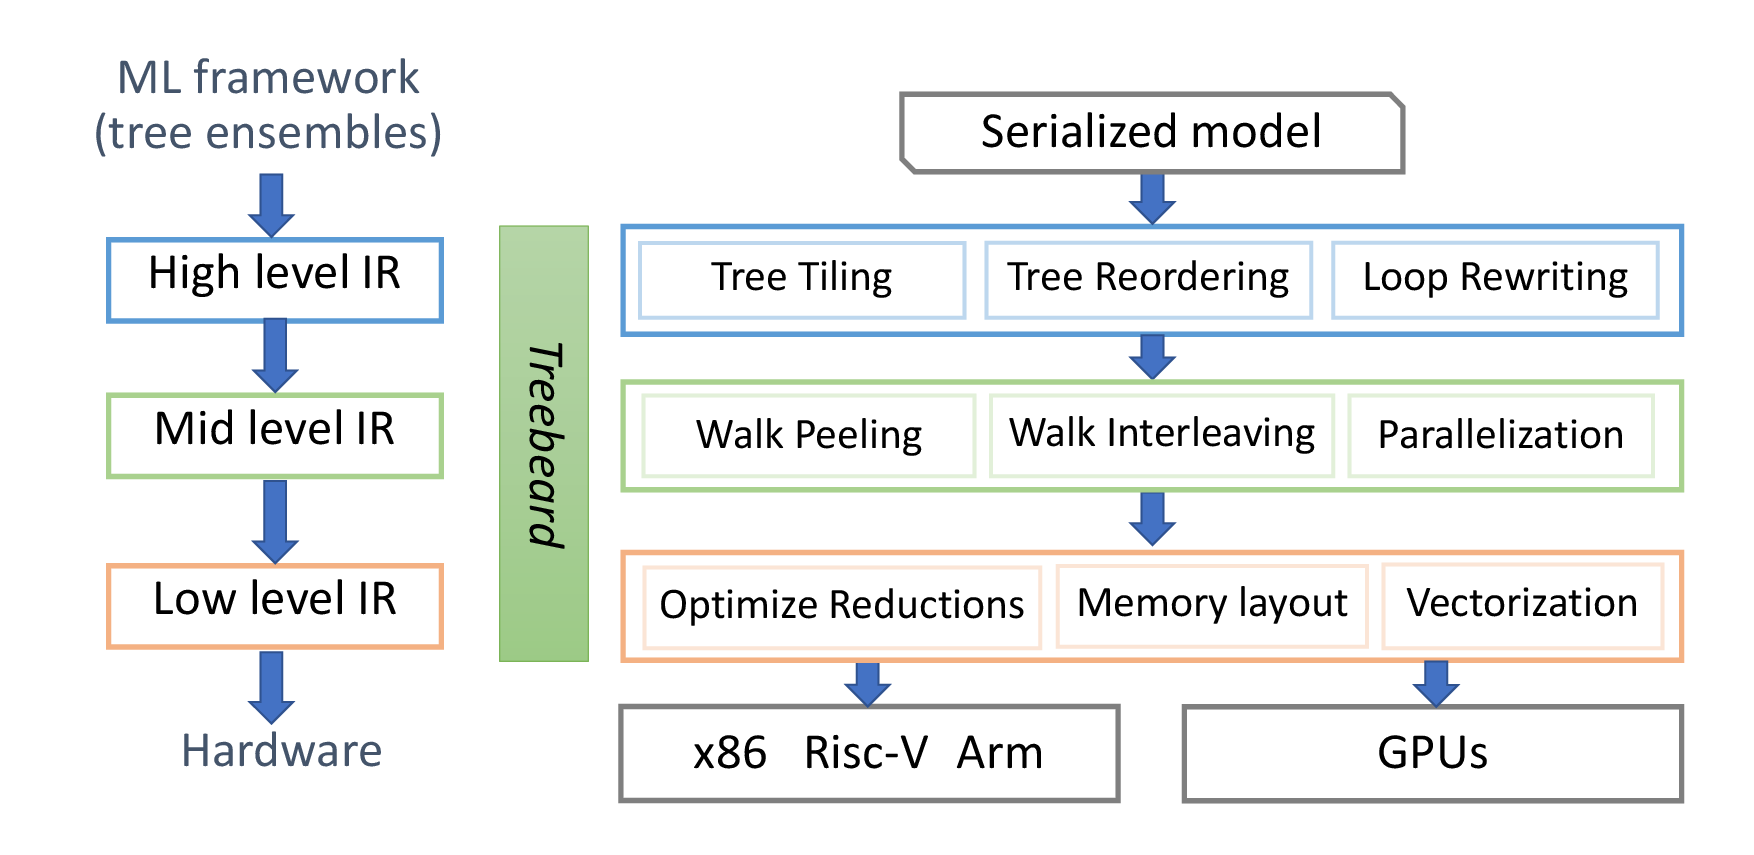
\includegraphics[width=\linewidth]{figures/compiler.png}
  \caption{\Treebeard{} compiler structure.}
  \label{Fig:CompilerStructure}
\end{figure}

% \begin{figure*}[htb]
%   \centering
%   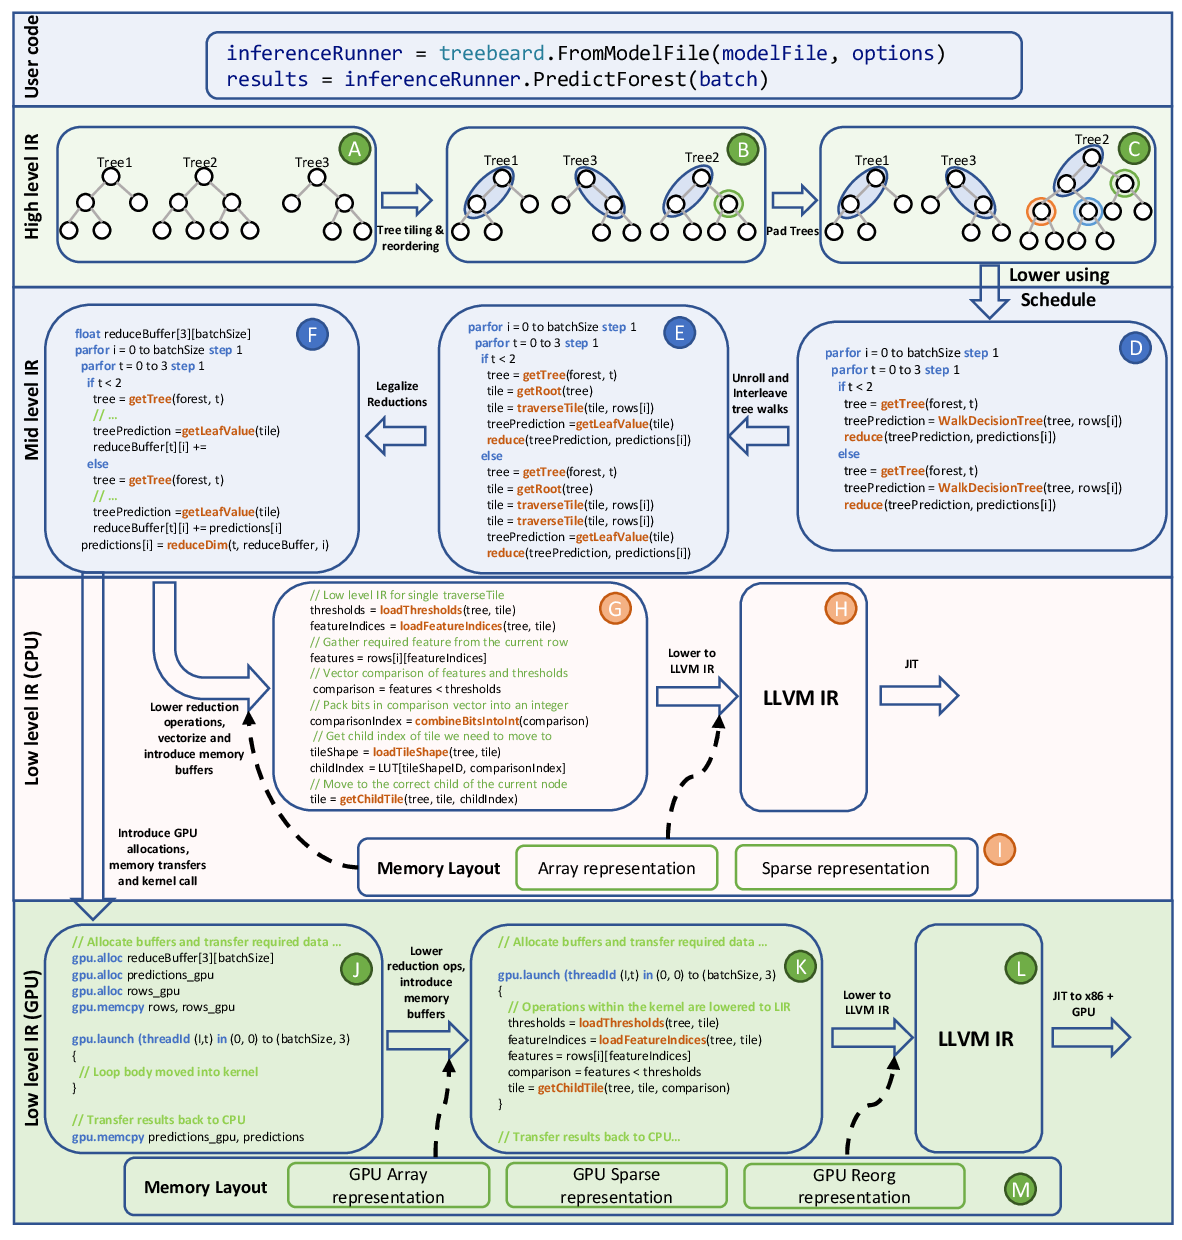
\includegraphics[width=\linewidth]{figures/OverviewExample_New.png}
%   \vskip 10pt
%   \caption{\Treebeard{} IR lowering and optimization details: the three abstraction levels in \Treebeard{}'s IR are shown. The
%            high level IR is a tree-based IR to perform model level optimization, the mid-level IR is for
%            loop optimizations that are independent of memory layout and the low level IR allows us to perform
%            vectorization and other memory layout dependent optimizations.}
%   \label{Fig:LoweringExample}
% \end{figure*}

\begin{figure*}[htb]
  \centering
  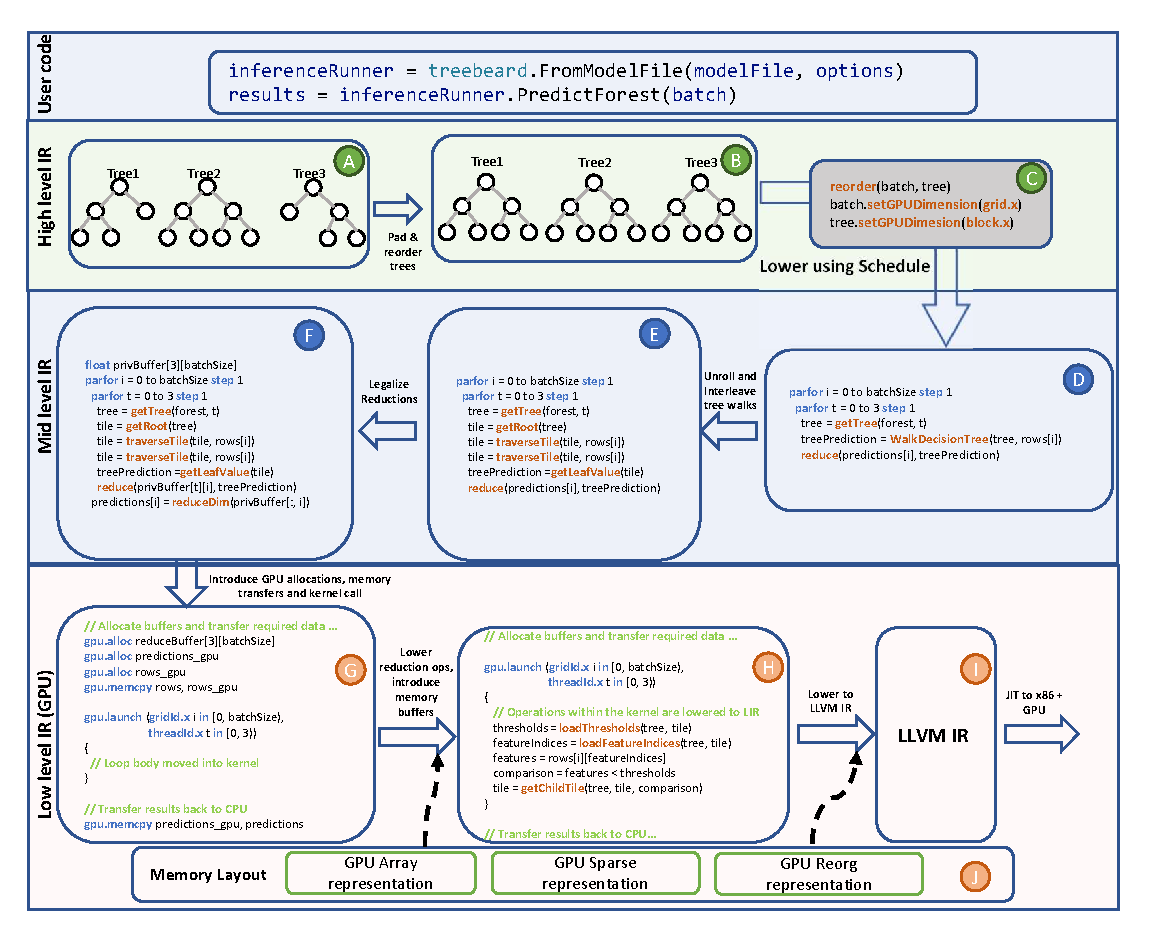
\includegraphics[width=\linewidth]{figures/GPUCompilationOverview-cropped.pdf}
  \vskip 10pt
  \caption{\Treebeard{} IR lowering and optimization details: the three abstraction levels in \Treebeard{}'s IR are shown. The
           high level IR is a tree-based IR to perform model level optimization, the mid-level IR is for
           loop optimizations that are independent of memory layout and the low level IR allows us to perform
           vectorization and other memory layout dependent optimizations.}
  \label{Fig:GPULoweringExample}
\end{figure*}

In HIR, the model is represented as a collection of binary trees. This abstraction
allows the implementation of optimizations that require the manipulation of the model
or its constituent trees. In Figure \ref{Fig:LoweringExample}, \circled{A}
shows this representation for a model with three trees. 
In HIR, \Treebeard{} tiles tree nodes together to convert
the binary tree to an n-ary tree as shown in \circled{B}. Trees are also 
reordered to enable better code generation and padded to allow more 
efficient traversal as shown in \circled{C}. While these are the optimizations currently 
implemented in \Treebeard{}, these are by no means the only ones that 
are enabled by HIR. It is not difficult to imagine optimizations 
such as tree pruning for specified accuracy levels for example.
These optimizations and rewrites that are performed on the domain-specific 
HIR would have been much on a traditional loop based IR or even in 
other IRs within \Treebeard{}.


After these model-level optimizations are performed on the HIR, the 
code is lowered to the mid-level IR (MIR) as dictated by a user specified schedule
(\circled{C} to \bluecircled{D}) in Figure \ref{Fig:LoweringExample}). The schedule specifies how
the iteration space that goes over the trees and input rows is to be traversed. 
It specifies how the iteration space is to be tiled, which loops are to be
parallelized, which loops are to be mapped to GPU grid and block dimensions etc.
(Details in Section \ref{Sec:SchedulingLang}). MIR is a loop-based IR that 
explicitly encodes details of the iteration space has to be traversed. However, 
it still abstracts details about the in-memory representation of the model. 
Optimizations such as tree-walk unrolling and interleaving are performed 
on the MIR (\bluecircled{E}). Subsequently, reduction operations are split and rewritten 
to correctly and explicitly implement reduction in the presence of 
parallel loops (\bluecircled{F}). More details of this process that we call 
\emph{legalization} are in Section \ref{Sec:Reduction}. Another important 
point to note is that MIR is independent of the target processor and therefore
all optimizations on MIR can be reused across CPU and GPU compilation.

The MIR is then further lowered to a low-level IR (LIR). This is the
level at which the compilation pipeline diverges for CPUs and GPUs. In 
the GPU compilation pipeline, the required memory transfers and kernel
invocations are inserted into the LIR (\circled{J}). Additionally, buffers 
to hold model values are inserted and tree operations are lowered to
explicitly refer to these buffers. This lowering is controlled by 
a plugin mechanism where different in-memory representations can 
be added to the compiler by implementing an interface. These plugins
provide information required for the lowering of MIR to LIR as well as 
the lowering to LLVM IR as shown in Figure \ref{Fig:LoweringExample}.
Again, a significant amount of code is shared between the
CPU and GPU pipelines for representations that are common between them
(Array and Sparse representations). Vectorization of tree traversals 
is also explicitly represented in LIR.

To reiterate, the following are the salient points of \Treebeard{}'s design.
\begin{enumerate}
  \item The compiler uses three intermediate representations (IRs) to
  represent the inference computation at different levels of abstraction. This
  allows different optimizations to be performed and also allows us to share
  infrastructure between compilation pipelines for different target processors.

  \item The specification of how the inference computation is to be lowered to 
  loops is not encoded directly in the compiler. Instead, this 
  is specified as an input to the compiler using a scheduling language that is 
  specialized for decision tree inference computations (Section \ref{Sec:SchedulingLang}).
  This separation allows us to build optimizations and schedule exploration 
  mechanisms independent of the core compiler (Section \ref{AutoTuneHeuristic}). 
  The scheduling language also exposes details like parallelization, optimization
  of reductions (vectorization, use atomics, shared memory on GPUs etc.).

  \item \Treebeard{} has been designed to keep the optimization passes and code 
  generator independent of the in-memory representation finally used for the model. To achieve 
  this, \Treebeard{} specifies an interface to implement that provides the necessary 
  capabilities to the code generator as a plugin. This interface abstracts several details
  on how model values are stored. In particular, it abstracts the actual layout of 
  the memory buffers, how to load model values like thresholds and feature indices, how 
  to move from a node to its children and determining whether a node is a leaf.
  This design allows us to write each memory representation as a standalone plugin 
  and reuse the rest of the compiler infrastructure.
\end{enumerate}
\section{Scheduling Language}
\label{sec:schedule}
As we articulated in Section \ref{sec:intro}, there are several 
different configurations and optimizations strategies for decision 
tree inference. The best ones are significantly different across
models, batch sizes and hardware platforms. Therefore, designing
any one hard-coded lowering strategy is not feasible as this would 
make portable performance impossible. To address this problem, we 
design a scheduling language for \Treebeard{}. The scheduling 
language provides an abstract way to specify loop structure and 
other optimizations as an input to the compiler. Making the 
scheduling specification external to the compiler allows to build 
auto-schedulers and auto-tuners (Section \ref{sec:exploring}).
Using a scheduling language will also significantly simplify 
adding support for new hardware as this will likely require
different locality optimizations and loop transformations.

The goal of \Treebeard{}'s scheduling language is to declaratively
express loop structures and the application of other optimizations 
(tree walk unrolling, tree walk interleaving etc.). 

\subsection{Language Definition}
The core construct of \Treebeard{}'s scheduling language is an 
\textbf{\emph{index variable}} which abstractly represents a loop. 
The language then provides directives to manipulate these index 
variables. There are two special index variables -- \op{batch} and
\op{tree} that are used to represent the batch and tree loops and all 
other index variables are derived from these. A schedule derives 
new index variables from these root index variables by applying
directives. 

\Treebeard{}'s scheduling language has three classes of directives. The first is a set 
of loop modifiers that are used to specify the structure of the loop nest to
walk the iteration space (Table \ref{Tab:LoopModifiers}). The second is a set of 
directives that enable optimizations on a loop (Table \ref{Tab:Optimizations}). 
Finally, we have a class of attributes that enable reduction specific optimizations
(Table \ref{Tab:ReductionOpts}).

% \subsubsection{Loop Modifiers}
% The clauses modify these index variables or 
% index variables derived from these (through the application of clauses).
% \begin{itemize}
%   \item \textbf{tile}: Tile the passed index variable using a fixed tile size.
%   \item \textbf{split}: Split the range of the passed index variable into two parts. The range of the first part is specified
%   by an argument.
%   % \item \textbf{unroll}: Unroll an index completely
%   \item \textbf{reorder}: Reorder the specified indices. The specified indices must be successive indices in the current loop nest.
%   \item \textbf{specialize}: Generate separate code for each iteration of the specified index variable. This is useful 
%   while parallelizing across trees and these trees have different depths.
%   \item \textbf{gpuDimension}: Maps the specified index variable to represent a dimension in either the GPU kernel grid or thread block.
% \end{itemize}

\begin{table}[htb]
  \centering
  \resizebox{\linewidth}{!}{
  \begin{tabularx}{\linewidth}{c | l | l}
   \toprule
   \textbf{Directive} & \textbf{Inputs} & \textbf{Description} \\
   \midrule
   \multirow{4}{*}{\texttt{tile}} & \textbf{indexVar}  & \multirow{4}{*}{\parbox{0.55\linewidth}{Tile the loop corresponding to \textbf{indexVar}
   with the specified tile size. Resulting loops will be represented by \textbf{outer} and \textbf{inner}.}} \\
                                               &  \textbf{outer} & \\
                                               &  \textbf{inner} &  \\
                                               &  \textbf{tileSize} &  \\
   \midrule
   \multirow{6}{*}{\texttt{split}} & \textbf{indexVar}  & \multirow{6}{*}{\parbox{0.55\linewidth}{Fiss the loop represented by \textbf{indexVar}
   at iteration \textbf{splitIter}. Resulting loops will be represented by \textbf{first} and \textbf{second}. Returns a maps from nested 
   index variables to new ones created by splitting.}} \\
                                               &  \textbf{first} & \\
                                               &  \textbf{second} &  \\
                                               &  \textbf{splitIter} &  \\
                                               & & \\
                                               & & \\

   \midrule
   \multirow{4}{*}{\texttt{reorder}} & \textbf{indices[]}  & \multirow{4}{*}{\parbox{0.55\linewidth}{Permute loops corresponding to the specified index variables.
   The loops must be perfectly nested in the current loop structure.}} \\
                                               &   & \\
                                               &   &  \\
                                               &   &  \\
   \midrule
   \multirow{4}{*}{\texttt{specialize}} & \textbf{indexVar}  & \multirow{4}{*}{\parbox{0.55\linewidth}{Generate specialized code for each iteration of the loop. 
   Useful when different iterations of a loop need to execute different code.}} \\
                                               &   & \\
                                               &   &  \\
                                               &   &  \\
   \midrule
   \multirow{3}{*}{\texttt{gpuDimension}} & \textbf{indexVar}  & \multirow{3}{*}{\parbox{0.55\linewidth}{Map the passed index variable to a dimension of either the grid
   or thread block.}} \\
                                               & \textbf{gpuDim}  & \\
                                               &   &  \\

  \bottomrule
  \end{tabularx}
  }
  \vskip 5pt
  \caption{\label{Tab:LoopModifiers} List of all the loop modifiers in \Treebeard{}'s scheduling language. We use \emph{index variable}
  and \emph{loop} interchangeably in descriptions for clarity of exposition.}
\end{table}


% The following are examples of how the loop modifiers can be used.
% \begin{itemize}
%   \item The loop order used by XGBoost\cite{XGBoost} is (tree, batch) -- walk one tree for all inputs in the batch before 
%   moving to the next tree. The corresponding schedule would be
% \begin{lstlisting}[style=c++]
%   reorder(tree, batch)
% \end{lstlisting}

%   \item The below schedule computes 2 trees at a time over the whole batch.
% \begin{lstlisting}[style=c++]
%   tile(tree, t0, t1, 2)
%   reorder(t0, batch, t1)
% \end{lstlisting}

%   \item If we additionally only want to compute over 4 input rows (rather than the whole batch) for
%   every 2 tree, and then move onto the next 2 trees for the same set of inputs, then the schedule is as follows. 
% \begin{lstlisting}[style=c++]
%   tile(batch, b0, b1, 4) 
%   tile(tree, t0, t1, 2)
%   reorder(b0, t0, b1, t1) 
% \end{lstlisting}

% \end{itemize}

% \subsubsection{Optimizations}
% The following clauses provide ways to optimize the inference routine being generated.
% \begin{itemize}
%   \item \textbf{cache}: Cache the working set of one iteration of the specified loop corresponding
%   to this index. This can be specified on either batch or tree loops. Specifying it 
%   on a batch loop leads to all rows accessed in a single iteration of the loop 
%   being cached. Similarly, specifying it on a tree loop leads to all trees accessed in 
%   one iteration of that loop being cached.
%   \item \textbf{parallel}: Execute the loop corresponding to this index in parallel.
%   \item \textbf{interleave}: Interleave the execution of the tree walks within the current index (must be applied on an inner most index).
%   \item \textbf{unrollWalk}: Unroll tree walks at the current index. 
%   \item \textbf{peelWalk}: Peel the first n steps of the specified tree walk and don't check for leaves for that number of steps.
% \end{itemize}

\begin{table}[htb]
  \centering
  \resizebox{\linewidth}{!}{
  \begin{tabularx}{\linewidth}{c | l | l}
   \toprule
   \textbf{Directive} & \textbf{Inputs} & \textbf{Description} \\
   \midrule
   \multirow{4}{*}{\texttt{cache}} & \textbf{indexVar}  & \multirow{4}{*}{\parbox{0.55\linewidth}{Cache the working set of one iteration of the specified loop. 
   Cache rows for a batch loop and trees for a tree loop.}} \\
                                               &  &  \\
                                               &  &  \\
                                               &  &  \\
   \midrule
   \multirow{2}{*}{\texttt{parallel}} & \textbf{indexVar}  & \multirow{2}{*}{\parbox{0.55\linewidth}{Execute the iterations of the specified 
   loop in parallel.}} \\
                                               &  & \\

   \midrule                                               
   \multirow{3}{*}{\texttt{interleave}} & \textbf{indexVar}  & \multirow{3}{*}{\parbox{0.55\linewidth}{Interleave tree walks within the specified 
   loop (must be innermost loop).}} \\
                                               &  & \\
                                               &  & \\

   \midrule                                               
   \multirow{3}{*}{\texttt{unrollWalk}} & \textbf{indexVar}  & \multirow{3}{*}{\parbox{0.55\linewidth}{Unroll tree walks at the specified loop 
   for \textbf{unrollDepth} hops. Loop must be an innermost loop.}} \\
                                               & \textbf{unrollDepth} & \\
                                               &  & \\

  \bottomrule
  \end{tabularx}
  }
  \vskip 5pt
  \caption{\label{Tab:Optimizations} List of optimization directives in \Treebeard{}'s scheduling language. 
  We use \emph{index variable} and \emph{loop} interchangeably in descriptions for clarity of exposition.}
\end{table}


% \subsubsection{Reduction Optimization}
% \begin{itemize}
%   \item \textbf{atomicReduce}: Use atomic memory operations to accumulate values across 
%   parallel iterations of the specified loop. 
%   \item \textbf{sharedReduce}: Only applies to GPU compilation. Specifies that intermediate
%   results are to be stored in shared memory.
%   \item \textbf{vectorReduce}: Use vector instructions with the specified vector width 
%   to reduce intermediate values across parallel iterations of the specified loop.
% \end{itemize}

\begin{table}[htb]
  \centering
  \resizebox{\linewidth}{!}{
  \begin{tabularx}{\linewidth}{c | l | l}
   \toprule
   \textbf{Directive} & \textbf{Inputs} & \textbf{Description} \\
   \midrule
   \multirow{3}{*}{\texttt{atomicReduce}} & \textbf{indexVar}  & \multirow{3}{*}{\parbox{0.55\linewidth}{Use atomic memory operations to accumulate values across 
   parallel iterations of the specified loop.}} \\
                                               &  &  \\
                                               &  &  \\
   \midrule
   \multirow{3}{*}{\texttt{sharedReduce}} & \textbf{indexVar}  & \multirow{3}{*}{\parbox{0.55\linewidth}{Specifies that intermediate
   results are to be stored in shared memory (GPU only).}} \\
                                               &  & \\
                                               &  & \\

   \midrule                                               
   \multirow{4}{*}{\texttt{vectorReduce}} & \textbf{indexVar}  & \multirow{4}{*}{\parbox{0.55\linewidth}{Use vector instructions with the specified vector width 
   to reduce intermediate values across parallel iterations of the specified loop.}} \\
                                               & \textbf{width} & \\
                                               &  & \\
                                               &  & \\

  \bottomrule
  \end{tabularx}
  }
  \vskip 5pt
  \caption{\label{Tab:ReductionOpts} List of reduction optimization directives in \Treebeard{}'s scheduling language. 
  We use \emph{index variable} and \emph{loop} interchangeably in descriptions for clarity of exposition.}
\end{table}


%\TODO{Add examples for RAPIDS, Tahoe (Maybe show some strategies can be encoded?)}

We now show how the implementation strategies of several existing systems can 
be encoded in \Treebeard{}'s scheduling language. First, we note that the 
default loop order is [\op{batch}, \op{tree}], i.e, for each row in the input
batch, go over all trees.

% \subsection{The XBoost Schedule}
XGBoost\cite{XGBoost} implements inference on the CPU by going 
over a fixed number of rows (64 in the previous version)
for every tree and then moving to the next tree. When all trees 
have been walked for this set of rows, the next set of rows is 
taken up. Also, different sets of rows are processed in parallel.
This schedule can be implemented in \Treebeard{}'s scheduling language 
as follows.
\begin{lstlisting}[style=c++]
  tile(batch, b0, b1, CHUNK_SIZE)
  reorder(b0, tree, b1)
  parallel(b0)
\end{lstlisting}

Tahoe\cite{Tahoe} has four strategies for inference on the GPU that it picks from for a given model. 
We show how two of these strategies can be encoded using \Treebeard{}'s scheduling language.
The rest can be encoded similarly. 
\begin{itemize}
  \item \textbf{Direct Method}: In this strategy, a single GPU thread walks all trees
  for a given input row. The schedule for this strategy is as follows.
\begin{lstlisting}[style=c++]
  tile(batch, b0, b1, ROWS_PER_TB)
  reorder(b0, b1, tree)
  gpuDimension(b0, grid.x)
  gpuDimension(b1, block.x)
\end{lstlisting}
  Here, \op{ROWS\_PER\_TB} is the number of rows that are processed by a single thread block.
  \item \textbf{Shared Data}: In this strategy, a thread block walks all the trees 
  for a given row in parallel. If threads walk multiple trees, each thread accumulates
  partial results. Finally, a thread block wide reduction is performed to compute 
  the prediction. The schedule for this strategy is as follows.
\begin{lstlisting}[style=c++]
  reorder(batch, tree)
  gpuDimension(batch, grid.x)
  gpuDimension(tree, block.x)
  cache(batch)
\end{lstlisting}
%   \item \textbf{Shared Forest}: In this strategy, the whole model is loaded into 
%   shared memory and subsequently, a single thread walks all trees for a particular
%   row. The schedule for this strategy is as follows.
% \begin{lstlisting}[style=c++]
%   tile(batch, b0, b1, ROWS_PER_TB)
%   tile(tree, t0, t1, N_TREES)
%   reorder(b0, b1, t0, t1)
%   cache(t0)
%   gpuDimension(b0, grid.x)
%   gpuDimension(b1, block.x)
% \end{lstlisting}
%   Here, we create a placeholder single iteration loop \op{t0} so that we can 
%   specify that all trees are to be cached.
%   \item \textbf{Shared Partial Forest}: In case the model is too large to fit into
%   shared memory, the model is split into chunks and each chunk is loaded into shared
%   memory. Again, as in the previous strategy, one thread walks all trees assigned to
%   a thread block for a row. The schedule for this strategy is as follows.
% \begin{lstlisting}[style=c++]
%   tile(batch, b0, b1, ROWS_PER_TB)
  
%   tile(tree, t0, t0Inner, TREES_PER_TB)
%   tile(t0Inner, t1, t2, TREES_PER_TB)
%   cache(t1)
%   reorder(b0, t0, b1, t1, t2)

%   gpuDimension(b0, grid.x)
%   gpuDimension(t0, grid.y)
%   gpuDimension(b1, block.x)
% \end{lstlisting}
\end{itemize}

There are some simplifying assumptions and limitations in the current design
of the scheduling language. Mainly, tree traversals are considered atomic and
accumulation of tree predictions is done immediately (as opposed to, 
for example, collecting all predictions and performing a reduction later).
However, we find that these are not significant limitations in practice as
the current design is able to express most strategies of interest.
\section{Overview of \Treebeard{} Multi-Level Compilation}

% \begin{itemize}
%   \item The compiler performs a number of optimizations on the HIR and MIR to improve the performance of the generated code.
%   \item Optimizations in HIR mainly transform the model itself. Tiling, tree reordering and padding are some of the 
%   optimizations that are performed on the HIR. \TODO{Should we use the MICRO paper overview for this part?}
%   \item Explain lowering to MIR using the schedule here.
%   \item Optimizations on the MIR include tree walk unrolling, tree walk interleaving, loop tiling, parallelization etc.
% \end{itemize}

\Treebeard{} takes a serialized decision tree ensemble as input (
XGBoost JSON, ONNX etc.) and automatically generates an optimized inference function
that can either target CPUs or GPUs. 
Figure \ref{Fig:CompilerStructure} shows the structure of the \Treebeard{} compiler. 
The inference computation is lowered through three intermediate representations
-- high-level IR (HIR), mid-level IR (MIR) and low-level IR (LIR). The LIR is
finally lowered to LLVM and then JIT'ed to the specified target processor. 
\Treebeard{} is built using the open-source \TreebeardOLD{} infrastructure~\cite{Treebeard}.
% Since the \TreebeardOLD{} infrastructure was originally designed to target CPUs,
% significant extensions were required to support schedule-guided compilation for CPUs and GPUs. 
The \TreebeardOLD{} infrastructure was originally designed to target CPUs.
It lacks a scheduling language and does not support generating code for 
different implementation strategies. We enhance \TreebeardOLD{}  
to support schedule-guided compilation for CPUs and GPUs.
The parts \Treebeard{} that are new or significantly different compared to \TreebeardOLD{}
are shown as shaded boxes in Figure \ref{Fig:CompilerStructure}.
% However, it implements several optimizations on the HIR and MIR that 
% can be leveraged across target processors and we find that some these 
% are beneficial for GPUs as well. 
% This reuse of optimizations is possible 
% because the intermediate representations on which these optimizations are performed 
% are abstract and are designed to be target-independent. We briefly review these 
% optimizations below. 

\begin{figure}[htb]
  \centering
  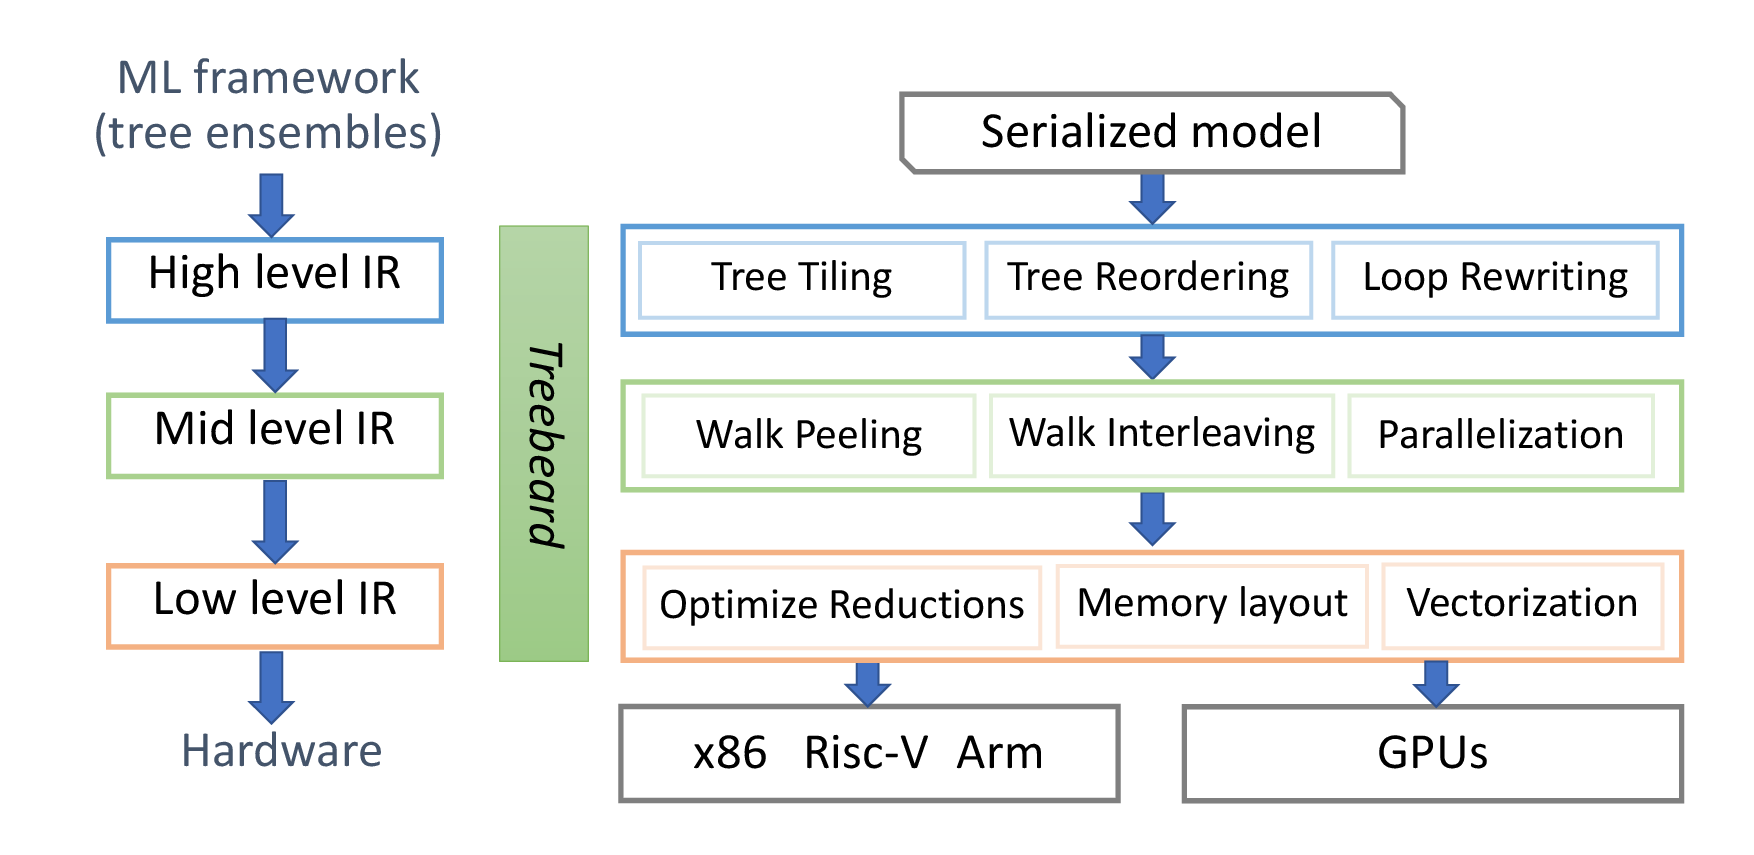
\includegraphics[width=\linewidth]{figures/compiler.png}
  \caption{\Treebeard{} compiler structure.}
  \label{Fig:CompilerStructure}
\end{figure}

Table \ref{Tab:IRSpecification} lists the operations in the three IRs. 
In HIR, the model is represented as a collection of binary trees. This abstraction
allows the implementation of optimizations that require the manipulation of the model
or its constituent trees. We extend the \TreebeardOLD{} infrastructure with loop rewrites on 
the HIR that are implemented through the scheduling language (Section \ref{sec:schedule}).
The \emph{schedule} is implemented as an MLIR attribute on the \op{predictEnsemble} operation.
We use this object to implement the automatic scheduling described in Section \ref{sec:exploring}. 
We reuse HIR transformations to reorder and pad trees from \TreebeardOLD{}.
The tree transformations that reorder and pad trees are used in conjunction 
with loop transformations like splitting to specialize inference code as the example 
in Section \ref{sec:motivation} shows. Also, we enable tree padding only if the schedule 
specifies unrolling of tree walks.
% Figure \ref{Fig:HIRExample} shows this representation for a model 
% with four trees and how the model can be transformed. The model contains two trees of 
% depth 1 and two trees of depth 2 (\circled{A}). The right side of the diagram shows the models after 
% padding and reordering (\circled{B}). Padding makes all leaves in a tree the same depth (Trees 2 and
% 4 are padded). Trees are reordered so that trees of the same depth are together (Trees 
% 2 and 3 are swapped). We use this model as a running example for the rest of the section.
% After these model-level optimizations are performed on the HIR, the 
% code is lowered to the mid-level IR (MIR) as dictated by a  
% \emph{\textbf{schedule}}. The schedule determines how to traverse
% the iteration space that goes over the trees and input rows 
% by specifying how loops are to be tiled, 
% parallelized, mapped to GPU grid and block dimensions etc.
% (Details in Section \ref{sec:schedule}). While MIR is a loop-based IR that 
% explicitly encodes details of the iteration space has to be traversed, 
% it still abstracts details about the in-memory representation of the model. 

The HIR is lowered to MIR as dictated by the \emph{schedule}.
Optimizations like tree-walk unrolling and tree-walk interleaving
are performed on the MIR. 
% These optimizations are beneficial for GPUs as well.
% and the design of \TreebeardOLD{} allows us to reuse the tree-walk 
% unrolling and tree-walk interleaving optimizations on the MIR for GPUs.
% While building \Treebeard{}, we found that
One surprising thing we found while developing \Treebeard{} was that 
we could use ILP to improve performance on GPUs. 
One of the performance bottlenecks in inference code targeted 
to GPUs was that warps spent significant time being stalled. We were able to 
alleviate this bottleneck by interleaving tree walks. 
% This significantly improved performance of generated 
% code. The fact that exploiting ILP improved performance on GPUs was surprising. 

In the generated MIR, the compiler uses the \op{reduce} op from 
the \op{reduction} dialect we design (details in Section \ref{sec:reduction})
to represent reduction operations. The lowering of the \op{reduce} operation 
involves introducing temporary buffers and splitting the operation  
to correctly implement reduction in the presence of 
parallel loops. This process, that we call \textbf{\emph{legalization}}, is 
described in Section \ref{sec:reduction}. 

% \TODO{Should we talk about how interleaving is implemented as a 
% statemachine and therefore it can be used across representations 
% and tile traversal techniques?}

The MIR is further lowered to a low-level IR (LIR). 
Significant changes to the original \TreebeardOLD{} design were required to get
LIR to correctly lower to GPU code. The most important of these was 
changing how the compiler implements support for in-memory 
representations of models (Section \ref{sec:representations}).
% With these design changes, we were able to reuse much of the CPU 
% implementation while customizing some parts for GPUs (for example,
% buffers need to be allocated differently for CPU and GPU, caching 
% is implemented differently etc.). 
Also, when the target processor is a GPU, the required memory transfers and kernel
invocations are inserted into the LIR. Additionally, buffers 
to hold model values are inserted and abstract tree operations are lowered to
explicitly refer to these buffers.
% This lowering is controlled by 
% a plugin mechanism which enables different in-memory representations to 
% be added to the compiler by implementing an interface 
% (Section \ref{sec:representations}). Vectorization of tree traversals
% is also explicitly represented in LIR.
Subsequently, the LIR is lowered to LLVM and then JIT'ed to the 
specified target processor.
% \subsection{Optimizations on High-Level IR}
% We augment the existing \TreebeardOLD{} infrastructure with loop rewrites on 
% the HIR that are implemented through the scheduling language (Section \ref{sec:schedule}).
% We use these to implement the automatic scheduling described in Section \ref{sec:exploring}. 
% Additionally, the \TreebeardOLD{} infrastructure implements HIR transformations to reorder and pad 
% trees. It also implements tree tiling transformations on the HIR \cite{Treebeard}. We reuse the 
% reordering and padding transformations on the HIR for GPUs. However, we found that 
% tiling trees was not beneficial for GPUs. This is because the tiling transformation
% introduces redundant computation inorder to vectorize computation on CPUs where 
% all lanes need to follow the same control flow. However, on SIMT GPUs, we find that 
% the benefits of tiling (coalescing memory accesses) do not outweigh the cost of
% redundant computation. We leave an investigation of this for future work.

% \subsection{Optimizations on Mid-Level IR}
% The original \TreebeardOLD{} infrastructure implements optimizations like 
% tree-walk unrolling, tree-walk interleaving, and parallelization
% on the MIR. These optimizations are beneficial for GPUs as well.
% and the design of \TreebeardOLD{} allows us to reuse the tree-walk 
% unrolling and tree-walk interleaving optimizations on the MIR for GPUs.

% While building \Treebeard{}, we found that one of the performance bottlenecks on the 
% GPU was that warps spent significant time being stalled. Since GPUs 
% implement scoreboarding~\cite{HennesseyPatterson}, we were able to alleviate this bottleneck by
% interleaving tree walks. This significantly improved performance of generated 
% code. We found it surprising that the use of ILP could benefit 
% performance on the GPU.  
% \TODO{Should we talk about how interleaving is implemented as a 
% statemachine and therefore it can be used across representations 
% and tile traversal techniques?}

% \subsection{A Note on Low-level IR}
% Significant changes to the original \TreebeardOLD{} design were required to get
% LIR to correctly lower to GPU code. The most important of these was 
% the change to how the compiler implements support for in-memory 
% representations of models (Section \ref{sec:representations}).
% With these design changes, we were able to reuse much of the CPU 
% implementation while customizing some parts for GPUs (for example,
% buffers need to be allocated differently for CPU and GPU, caching 
% is implemented differently etc.). 
% \section{\Treebeard{} IR Description}

% \begin{table*}[htb]
%   \centering
%   \resizebox{\linewidth}{!}{
%   \begin{tabularx}{\linewidth}{c l l l l}
%    \toprule
%    \textbf{Operation} & \textbf{Inputs} & \textbf{Outputs} & \textbf{Attributes} & \textbf{Description} \\
%    \midrule
%    \multirow{4}{*}{\texttt{predict\_ensemble}} & \textbf{data} & \textbf{result} & \textbf{ensemble} & Performs inference on the \textbf{data} using the model specified by\\
%                                                &               &                 & \textbf{predicate} & the \textbf{ensemble} attribute. The \textbf{schedule} attribute contains the \\
%                                                &               &                 & \textbf{schedule} & schedule described in Section \ref{sec:schedule}. \textbf{predicate} specifies the \\
%                                                 &               &                &                   & operator to use to evaluate nodes (Eg: $<$, $\leq$). \\
%    \midrule
%    \multirow{3}{*}{\texttt{walk\_decision\_tree}} & \textbf{trees[]} & \textbf{results[] }& \textbf{predicate}   & Represents an interleaved walk on all the element-wise pairs  \\ 
%                                                   & \textbf{rows[]}  &                    & \textbf{unrollDepth} & of \textbf{trees} and \textbf{rows}. \textbf{unrollDepth} specifies the number of \\
%                                                   &                  &                    &                      & hops to unroll. An array of tree walk results is returned.\\
%    \bottomrule
%   \end{tabularx}
%   }
%   \vskip 5pt
%   \caption{\label{Tab:Benchmarks}List of benchmark datasets and their parameters. 
%   The column \op{Leaf-biased} reports the number of leaf-biased trees per benchmark with $\langle\alpha =0.075, \beta =0.9 \rangle$. }
% \end{table*}

\begin{table*}[htb]
  \centering
  \resizebox{\linewidth}{!}{
  \begin{tabularx}{\linewidth}{c | l | l | l | l}
   \toprule
   \textbf{Operation} & \textbf{Inputs} & \textbf{Outputs} & \textbf{Attributes} & \textbf{Description} \\
   \midrule
   \multirow{4}{*}{\texttt{predictEnsemble}} & \textbf{rows[]} & \textbf{result} & \textbf{ensemble} & \multirow{4}{*}{\parbox{0.47\linewidth}{Performs inference on the data in \textbf{rows[]} 
                                                                                                     using the model specified by
                                                                                                     the \textbf{ensemble} attribute. The \textbf{schedule} attribute contains the 
                                                                                                     schedule described in Section \ref{sec:schedule}. \textbf{predicate} specifies the
                                                                                                     operator to use to evaluate nodes (Eg: $<$, $\leq$).}} \\
                                               &               &                 & \textbf{predicate} & \\
                                               &               &                 & \textbf{schedule} &  \\
                                               &               &                 &                   &  \\
   \midrule
   \midrule

   \multirow{3}{*}{\texttt{walkDecisionTree}} & \textbf{trees[]} & \textbf{results[] }& \textbf{predicate}   & \multirow{3}{*}{\parbox{0.47\linewidth}{Represents an interleaved walk on all the element-wise pairs 
                                                                                                                    of \textbf{trees} and \textbf{rows}. \textbf{unrollDepth} specifies the number of
                                                                                                                    hops to unroll. An array of tree walk results is returned.}} \\
                                                  & \textbf{rows[]}  &                    & \textbf{unrollDepth} &  \\
                                                  &                  &                    &                      & \\
   \midrule
   \multirow{2}{*}{\texttt{ensemble}} &  & \textbf{ensemble} & \textbf{model} & \multirow{2}{*}{\parbox{0.47\linewidth}{Represents the forest of trees that constitute the model. The   
                                                                                                                       \textbf{model} attribute contains the actual trees model.}} \\
                                      &  &                 &   & \\
   \midrule
   \multirow{2}{*}{\texttt{getTree}} & \textbf{ensemble} & \textbf{tree} &  & \multirow{2}{*}{\parbox{0.47\linewidth}{Get the tree at the specified index (\textbf{treeIndex}) from the \textbf{ensemble}.}} \\   
                                                                                                                       
                                      & \textbf{treeIndex} &                 &   & \\                                                                                                                       

   \midrule
   \multirow{2}{*}{\texttt{getTreeClassId}} & \textbf{ensemble} & \textbf{classId} &  & \multirow{2}{*}{\parbox{0.47\linewidth}{Get the class ID for the tree at index \textbf{treeIndex} 
                                                                                                                               in the \textbf{ensemble}. This is used for multi-class models.}} \\    
                                            & \textbf{treeIndex} &                 &   & \\                                                                                                                       

   \midrule
   \multirow{1}{*}{\texttt{getRoot}} & \textbf{tree} & \textbf{rootNode} &  & \multirow{1}{*}{\parbox{0.47\linewidth}{Get the root node of the specified tree.}} \\   

   \midrule
   \multirow{2}{*}{\texttt{isLeaf}} & \textbf{tree} & \textbf{bool} &  & \multirow{2}{*}{\parbox{0.47\linewidth}{Returns a boolean value indicating whether \textbf{node} is a leaf of \textbf{tree}.}} \\   
                                    & \textbf{node} &                 &   & \\                                                                                                                       

   \midrule
   \multirow{2}{*}{\texttt{getLeafValue}} & \textbf{tree} & \textbf{value} &  & \multirow{2}{*}{\parbox{0.47\linewidth}{Returns the value of the leaf \textbf{node} in \textbf{tree}.}} \\   
                                    & \textbf{node} &                 &   & \\                                                                                                                       

   \midrule
   \multirow{3}{*}{\texttt{traverseTreeTile}} & \textbf{trees[]} & \textbf{nodes[] }& \textbf{predicate}   & \multirow{3}{*}{\parbox{0.47\linewidth}{Represents an interleaved traversal of the   
                                                                                                                    nodes in \textbf{nodes} based on the data in \textbf{rows}. \textbf{predicate} specifies 
                                                                                                                    the operator to use to evaluate nodes.}} \\
                                                  & \textbf{nodes[]}  &             &               &  \\
                                                  & \textbf{rows[]}   &             &               & \\

   \midrule
   \multirow{3}{*}{\texttt{cacheTrees}} & \textbf{ensemble} & \textbf{ensemble}&     & \multirow{3}{*}{\parbox{0.47\linewidth}{Cache the trees in the \textbf{ensemble} between the specified \textbf{start} and \textbf{end} indices.   
                                                                                                                    The returned \textbf{ensemble} has the specified trees cached.}} \\
                                                  & \textbf{start}  &             &               &  \\
                                                  & \textbf{end}   &             &               & \\

   \midrule
   \multirow{3}{*}{\texttt{cacheRows}} & \textbf{rows[]} & \textbf{cachedRows[]}&     & \multirow{3}{*}{\parbox{0.47\linewidth}{Cache the rows in \textbf{rows[]} between the specified \textbf{start} and \textbf{end} indices.   
                                                                                                                    Returns an array of cached rows \textbf{cachedRows[]}.}} \\
                                                  & \textbf{start}  &             &               &  \\
                                                  & \textbf{end}   &             &               & \\

   \midrule
   \midrule
   \multirow{3}{*}{\texttt{loadThreshold}} & \textbf{buffer} & \textbf{threshold}&     & \multirow{3}{*}{\parbox{0.47\linewidth}{Load the threshold value for the node specified by \textbf{nodeIndex} 
                                                                                                                                      in the tree specified by \textbf{treeIndex} from \textbf{buffer}.
                                                                                                                                      Returns the loaded threshold.}} \\   
                                                  & \textbf{treeIndex}  &             &               &  \\
                                                  & \textbf{nodeIndex}   &             &               & \\

   \midrule
   \multirow{3}{*}{\texttt{loadFeatureIndex}} & \textbf{buffer} & \textbf{threshold}&     & \multirow{3}{*}{\parbox{0.47\linewidth}{Load the feature index for the node specified by \textbf{nodeIndex} 
                                                                                                                                      in the tree specified by \textbf{treeIndex} from \textbf{buffer}.
                                                                                                                                      Returns the loaded feature index.}} \\   
                                                  & \textbf{treeIndex}  &             &               &  \\
                                                  & \textbf{nodeIndex}   &             &               & \\

  \bottomrule
  \end{tabularx}
  }
  \vskip 5pt
  \caption{\label{Tab:IRSpecification} List of all the operations in the \Treebeard{} MLIR dialect. These operations are used 
  in conjunction with operations from other MLIR dialects like \op{scf}, \op{arith}, \op{gpu} etc. to represent and optimize 
  decision tree inference.}
\end{table*}

\section{Representing and Optimizing Reductions}
\label{sec:reduction}
\Treebeard{} needs to sum up individual tree predictions to compute 
the prediction of the model while performing inference. However,
generating fused reductions within arbitrary loop nests specified 
using \Treebeard{}'s scheduling language is non-trivial. We found 
that existing reduction support in MLIR is insufficient to code
generate and optimize these reductions. MLIR only supports reductions
of value types and does not provide ways to lower reductions to GPUs. 
To address this gap, we design an MLIR dialect that allows us to
specify accumulating values into an element of a multi-dimensional array
and can be lowered to CPU or GPU. 

The main abstraction we introduce is the \op{reduce} op. It models 
atomically accumulating values into an element of a 
multi-dimensional array (represented by an MLIR \op{memref}).
Consider the following \Treebeard{} schedule.
In our example, \op{N\_t} is the number of trees 
and \op{batch\_size} is the batch size. The schedule tiles the 
tree loop and parallelizes the resulting outer loop.
\begin{lstlisting}[style=c++]
  tile(tree, t0, t1, N_t/2);
  reorder(t0, t1, batch);
  parallel(t0);
\end{lstlisting}

The MIR generated by \Treebeard{} for the above schedule is as follows. 
\begin{lstlisting}[style=c++]
  float result[batch_size]
  model = ensemble(...) 
  par.for t0 = 0 to N_t step N_t/2:
    for t1 = 0 to N_t/2:
      for batch = 0 to batch_size:
        t = getTree(model, t0 + t1) 
        p = walkDecisionTree(t, rows[batch])
        reduce(result[batch], p)
\end{lstlisting}

The compiler simply generates a \op{reduce} op to perform
the required parallel reduction. 
The semantics of the \op{reduce} op is exactly the semantics of 
an atomic accumulation, i.e. it guarantees that all accumulations 
are correctly performed even in the presence of parallel loops. 
The \op{reduce} op is defined for all associative and commutative
reduction operations with a well-defined initial value. The 
reduction operator and the initial value are attributes applied
on the \op{reduce} op. 

Having modeled the reductions with an abstract operation, the 
aim now is to lower this to a correct and optimized 
implementation on both CPU and GPU. In order to do this, we 
first determine if any parallel loop iterations can accumulate 
into the same array element. We call such loops 
\emph{\textbf{reduction loops}}. If such loops exist, we 
\textbf{\emph{privatize}} the array for each iteration of the
loop. We call this process \textbf{\emph{legalization}}.
Subsequently, each privatized dimension 
can be reduced at the end of the reduction loop it was inserted for. 
%\TODO{We cannot do better than this in terms of memory usage} \TODO{Need a proof}.

In our example, \Treebeard{} determines that the \op{t0} loop is a reduction 
loop w.r.t the \op{result} array and therefore legalizes 
the reduction by inserting a privatized array 
\op{partResults}. The privatized dimension of this array 
is reduced at the end of the \op{t0} loop.

\begin{lstlisting}[style=c++]
  float result[batch_size], partResults[2][batch_size]
  model = ensemble(...) 
  par.for t0 = 0 to N_t step N_t/2:
    for t1 = 0 to N_t/2:
      for batch = 0 to batch_size:
        t = getTree(model, t0 + t1) 
        p = walkDecisionTree(t, rows[batch])
        reduce(partResults[t0/(N_t/2)][batch], p)
  
  results = reduceDimension(partResults[:, :], 0)
\end{lstlisting}

The op \op{reduceDimension} reduces values across the specified
dimension of an n-dimensional array. Here, 
it reduces all elements of the first dimension (dimension 0). 
and produces a result memref with a single dimension of size \op{batch\_size}.

To reduce the amount of memory used by arrays introduced for reduction,
we introduce the \op{reduceDimInplace} operation. It is similar to the 
\op{reduceDimension} op except that it updates the input array inplace
rather than writing results to a target array. It writes results to the 
zeroth index of the dimension being reduced. We use this op to 
compute intermediate results when several reduction loops are identified.

% \begin{definition}
%  \textbf{\op{reduce\_dimension\_inplace(memref, dim, [indices], [rangeStart], [rangeEnd])}}:
%   Computes the reduction over the dimension specified by \op{dimension} and stores the 
%   result at index 0 of that dimension. \op{[indices]} must be a vector of \op{dim} elements
%    (or empty if the dimension being reduced is the first dimension). \op{[rangeStart]} 
%    and \op{[rangeEnd]} must have the same number of elements. If both are \op{null} (not passed), 
%    all elements of the corresponding dimension are reduced. 
  
%   The computation performed by the op is defined by the following equation.
  
%   $memref[\vec{\boldsymbol{indices}}, 0, \vec{\boldsymbol{k}}] = \sum_{i=0}^{shape[dim]} memref[\vec{\boldsymbol{indices}}, i, \vec{\boldsymbol{k}}]\quad   \forall \vec{\boldsymbol{k}} \in \left[[rangeStart_0, rangeEnd_0), ... , [rangeStart_n, rangeEnd_n)\right]$  
% \end{definition}

\subsection{Lowering Reduction Operations}
% We implement lowering of the operations defined above to both the CPU and GPU.
% Since the lowering pipeline from MIR to LIR are different for CPU and GPU 
% compilation, we implement lowering and optimization of our reduction dialect to CPUs and
% GPUs simply using different MLIR rewrite patterns. 
In this section, we briefly describe 
how we lower the reduction operations to the CPU and GPU. 

For both CPU and GPU, \op{reduce} is lowered to a sequence 
of load, compute and write operations. This is possible because 
legalization ensures that parallel threads do not write to the same 
array element. 
%\subsubsection{Lowering to CPU}

For CPUs, we lower \op{reduceDimInplace} and 
\op{reduceDimension} to a simple loop nest that goes over the specified
subset of the input array, performs the reduction and writes 
the result into the appropriate location of the target array. 
If the schedule specifies that the reduction is to be vectorized,
the lowering passes generate vector (LLVM IR) instructions for 
the reduction.
% then as many elements as specified by the vector width are read 
% from the input array as a vector, accumulated as a vector, and 
% finally written back to the target array.

% In general, this works 
% well because reductions are typically being performed on dimensions
% other than the inner-most dimension and therefore, this strategy
% loads successive elements from memory maximizing memory bandwidth 
% utilization. 

% \TODO{explain atomic reduction}

% \subsubsection{Lowering to GPU}
The same reduction abstractions can be lowered to efficient GPU implementations
and therefore, simplify higher-level code generation. 
% The lowering for 
% the inplace and non-inplace operations are essentially the same, except 
% for the target array and we do not distinguish between them except 
% for finally storing the result. 
%
% The lowering of the \op{reduceDim*} 
\Treebeard{} can lower these ops to either exploit
parallelism across the independent reductions or 
the inherent parallelism in the reduction by performing a divide and conquer 
reduction depending on whether there are enough independent reductions to keep all threads
in a thread block busy.
% then the lowering pass can generate code that performs one (or 
% multiple) reductions in each thread. If, however, there are not 
% enough independent reductions, then the lowering pass generates a tree 
% style reduction where multiple threads cooperate to perform a single reduction
% using inter-thread shuffles.

% Another feature specific to GPU reductions is the use of shared memory. 
Additionally, if the schedule specifies that the reduction needs to be performed 
using shared memory, the privatized buffer is allocated in shared memory. 
% The compiler only allocates as much shared memory 
% as needed to hold values processed by a single thread-block.
%  and 
% index offsets are appropriately rewritten to handle the differences between 
% the indexing of the target memref and the shared memory array.
Our abstractions for reductions allow our lowering passes to be 
agnostic of whether we use shared memory and therefore allow 
us to enable or disable shared memory use independently from the other 
parts of the compiler. 

% We find that our current implementation of lowering reduction operations 
% is sufficient for \Treebeard{} and reduction is not the bottleneck in the
% generated code. However, we believe this approach to enabling 
% higher level code generators to easily generate reductions 
% through simple abstractions and then having the compiler 
% automatically lower them to efficient implementation is an
% important area for future work with applicability in several 
% domains. 

%\TODO{Should we mention how we handle multi-class models?}
\section{Representations}
\label{sec:representations}

The design of the \Treebeard{} compiler allows the implementation of different strategies for 
the in-memory representation of the model. The compiler currently has implementations for 
the three representations shown in Figure \ref{Fig:Representations}. The array and sparse 
representations are the ones described in the \Treebeard{} paper\cite{Treebeard}. The reorg 
representation is the representation used by the RAPIDs library\cite{RAPIDs}. 
The \textbf{array representation} is the simplest representation where the trees are stored in an array
in level order. The \textbf{sparse representation} stores the trees in a sparse format where only the
non-zero nodes are stored and nodes contain pointers to their children. The \textbf{reorg representation}
interleaves the array representation of each tree in the model: all root nodes are stored first, then 
the left children of all the roots and so on.
\begin{figure}[htb]
  \centering
  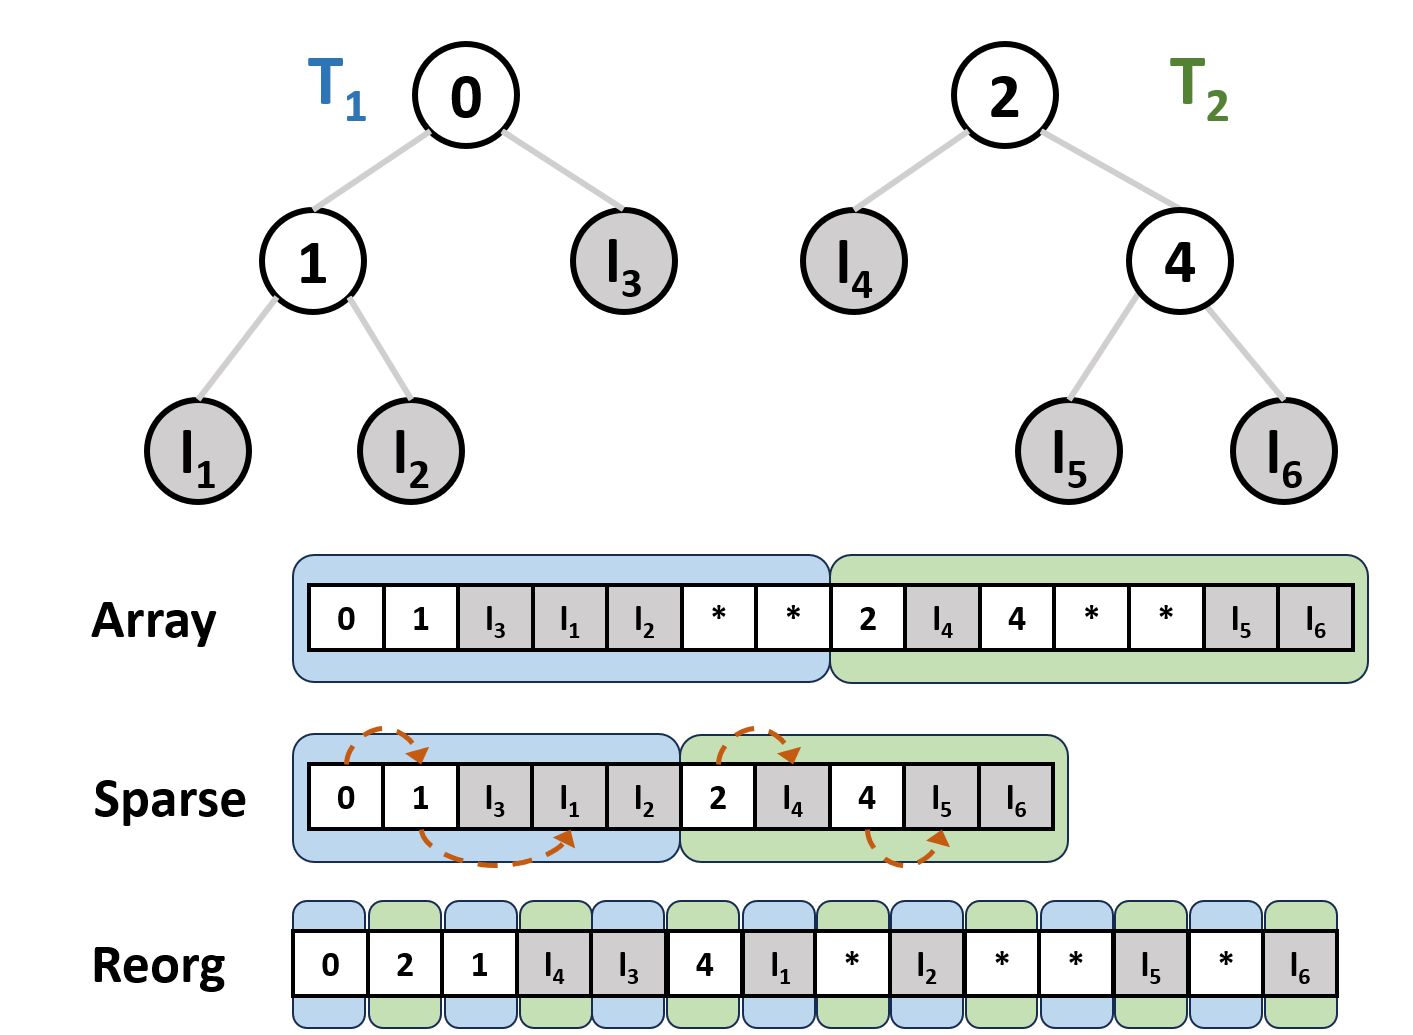
\includegraphics[width=\linewidth]{figures/representations.png}
  \caption{The three representations supported by \Treebeard{}.}
  \label{Fig:Representations}
\end{figure}

One of the major changes we make to the original design of \Treebeard{} \cite{Treebeard} is to
separate the implementation of representations from the rest of the compiler. This allows
us to implement representations as plugins to the compiler. We do this by defining an interface 
that each representation needs to implement. The code generator is implemented using methods 
on the representation interface thus hiding details of the actual representation from the core 
compiler. The interface abstracts the following details. 
\begin{itemize}
  \item \textbf{Buffer allocation:} The representation object exposes methods that generate 
  buffer allocations in the IR. 
  \item \textbf{Moving to child nodes:} Given the value of the predicate at a node (or tile),
  generate code to move to the appropriate child node of the current node.
  \item \textbf{Details of leaves:} The interface abstracts determining whether the current
  node is a leaf (which is needed to terminate walks) and how to get the value of the leaf
  (which is needed to get a tree's prediction).
  \item \textbf{Caching trees:} Since reading the trees into shared memory on GPU (or prefetching)
  them on CPU require knowledge of the buffer layout, the task of generating caching code for trees
  is delegated to the representation object. 
  \item \textbf{Loading thresholds and feature indices:} The representation object provides MLIR 
  rewrite patterns to lower operations that load thresholds and feature indices to LLVM IR. This
  is necessary because the details of how to load the thresholds and feature indices from the model 
  buffers is representation-specific.
\end{itemize}

In summary, the representation interface abstracts the details of how the model is stored in memory
and allows the compiler to generate code without having to explicitly know the details of the
representation. This design allows us to implement new representations without changing the core
compiler infrastructure. Implementing the representations as plugins also allows us to reuse
the implementations across different lowering pipelines. For example, the code for the array 
and sparse representations is almost fully shared between the CPU and GPU lowering pipelines.   

\section{Caching Implementation}
\label{sec:caching}

% \begin{itemize}
%   \item The compiler exposes caching of both trees and input rows in a unified manner.
%   \item This is independent of the final target on which the inference is to be run.
%   \item The caching is done at the granularity of a tree or a row.
%   \item Caching is encoded in the mid-level IR using the \op{cacheTrees} and \op{cacheRows} operations. 
%   These operations are generated when the HIR lowered to MIR and \op{Cache()} is specified on an 
%   index variable in the schedule. While the HIR is being lowered and a cached index variable is 
%   encountered, the compiler generates a \op{cacheTrees} or \op{cacheRows} operation depending on 
%   whether the index variable is a tree or a batch index variable.
%   \TODO{Should we talk about how the lowering from HIR to MIR is actually implemented as a tree walk?}
%   \item The lowering of these ops is done by the target-specific code generator.
%   \item For the \op{cacheRows} operation, \Treebeard{} uses pre-implemented lowerings for both
%   CPU and GPU. This is possible because the input is currently assumed to be a dense 
%   array format. 
%   \item For the \op{cacheTrees} operation, the lowering is representation-specific.
%   Each representation provides a lowering to the target-specific code generator
%   to lower the \op{cacheTrees} op when that representation is used.
%   \item The cache operations are lowered to reads into shared memory while compiling to GPU 
%   and to prefetches while compiling to CPU.
% \end{itemize}

\Treebeard{} provides mechanisms to cache both trees and input rows 
on both the CPU and GPU. As described in Section \ref{sec:schedule}, 
the user can specify that the working set of an iteration of an index
variable needs to be cached using the \op{Cache()} directive. This 
provides a unified way to specify caching of both trees and input rows.

\Treebeard{} implements caching at the granularity of a tree or a row.
Also, the semantics of caching depends on the target processor. For the CPU,
caching is implemented as prefetching, while for the GPU, caching is implemented
using shared memory.

\subsection{IR Representation of Caching}
Caching is encoded in the mid-level IR using the \op{cacheTrees} and \op{cacheRows} operations. 
These operations are generated when the HIR lowered to MIR and \op{Cache()} is specified on an 
index variable in the schedule. While the HIR is being lowered and a cached index variable is 
encountered, the compiler generates a \op{cacheTrees} or \op{cacheRows} operation depending on 
whether the index variable is a tree or a batch index variable. Additionally, as a part of the 
lowering process, \Treebeard{} determines the working set of the loop with caching enabled 
and generates a caching operation with the appropriate limits.

Each of the caching operations take parameters that specify the set of trees or rows that need 
to be cached. The caching operations are defined as follows. 
\begin{itemize}
  \item \textbf{\op{cacheTrees(forest, start, end)}:} This operation caches the trees in ensemble
  \op{forest} from \op{start} to \op{end}. The trees are cached in the order in which they are
  specified in the ensemble. 
  \item \textbf{\op{cacheRows(data, start, end)}:} This operation caches the rows in the input 
  array \op{data} from \op{start} to \op{end}. The rows are cached in the same order as in the
  input array.
\end{itemize} 

\subsection{Lowering of Caching Operations}
When the MIR is lowered to LIR, the cache ops are lowered to target-specific code. Each of 
the two caching operations is lowered differently for the CPU and the GPU.

For the \op{cacheRows} operation, \Treebeard{} uses pre-implemented lowerings for both
CPU and GPU. This is possible because the input is currently assumed to be a dense
array format. Therefore, regardless of any other configuration choices (like what representation 
is used for the model itself), the lowering of the \op{cacheRows} operation is the same. 
For the CPU, the \op{cacheRows} operation is lowered to prefetches. For the GPU, a 
series of coalesced loads read the rows into shared memory.

For the \op{cacheTrees} operation, the lowering is representation-specific. Each representation
provides a lowering to the target-specific code generator to lower the \op{cacheTrees} op when
that representation is used. However, the \Treebeard{} infrastructure does provide helpers 
to generate caching code to cache contiguous regions of memory. These helpers are reused 
as required across different representations. 

\section{Exploring the Schedule Space}
\label{sec:exploring}

% \begin{itemize}
%   \item The scheduling language described in Section \ref{sec:schedule} allows
%   for numerous possible schedules for a given model. 
%   Finding a schedule with good performance is a non-trivial task.
%   \item We identify a reasonable template schedule for GPUs which encompasses
%   all strategies published in prior work.
%   \item Describe the template schedule.
%   \item Even within the variants of this template schedule, there is a significant 
%   amount of variation in performance. Show the histogram. 
%   \item Extensively exploring all possible parameter values for the template schedule 
%   is infeasible due to the large number of parameters.
%   Cite some numbers on how long it takes to explore the schedule space.
%   \item List the observations we make and the heuristic we design based on these.
% \end{itemize}

The set of schedules that can be constructed using the scheduling language described in 
Section \ref{sec:schedule} is vast. Searching this schedule space to find a schedule that
provides good performance is a non-trivial task. To simplify this process, we identify a
template schedule for GPUs that encompasses several strategies published in prior work.
Our template schedule assigns a fixed number of rows to each thread block and to each thread.
It distributes the trees across a fixed number of threads and can cache trees and 
input rows if required. Unrolling and interleaving of tree walks is also supported.

The template schedule exposes a number of parameters that can be tuned to find a 
high-performance schedule.
\begin{itemize}
  \item \textbf{Number of rows per thread block (Integer):} The number of rows that are processed by each thread block.
  \item \textbf{Number of rows per thread (Integer):} The number of rows processed by each thread.
  \item \textbf{Number of tree threads (Integer):} The number of threads across which the trees are distributed.
  \item \textbf{Cache rows (Boolean):} Whether the input rows are cached in shared memory.
  \item \textbf{Cache trees (Boolean):} Whether the trees are cached in shared memory.
  \item \textbf{Unroll walks (Boolean):} Whether the tree walks are unrolled.
  \item \textbf{Tree walk interleave factor:} The number of tree walks that are interleaved.
  \item \textbf{Shared memory reduction:} Whether the reduction across tree threads is done in shared memory.
\end{itemize}

While the template schedule simplifies optimization of generated inference code, it is 
important to note that the \Treebeard{} compiler itself does not place any 
restrictions on the schedule. The user is free to specify any schedule they wish.
The auto-scheduler that implements the template schedule is implemented as a 
module outside the core \Treebeard{} compiler. Users are also free to implement 
other auto-schedulers that generate schedules different from the template schedule.

\begin{figure}[htb]
  \centering
  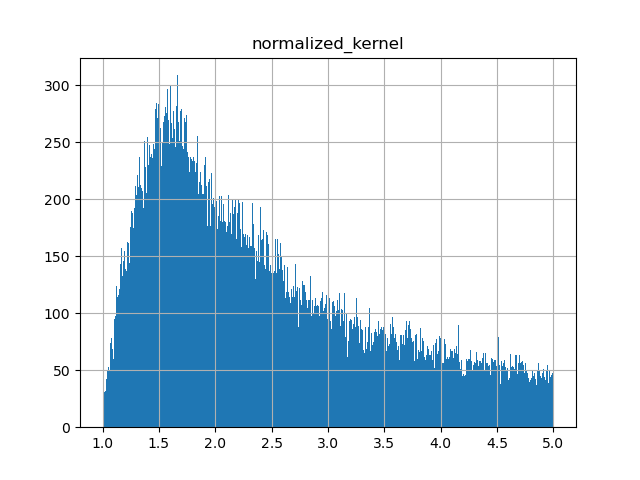
\includegraphics[width=\linewidth]{figures/normalized_kernel_histogram_lt5.png}
  \caption{Distribution of normalized execution times for all benchmark models
  with different parameter values for the template schedule. \TODO{We need to 
  describe exactly what the considered set of parameter values are.}}
  \label{Fig:ExecTimeDistribution}
\end{figure}

Figure \ref{Fig:ExecTimeDistribution} shows the distribution of normalized execution times
for all benchmark models with different parameter values for the template schedule.
The normalized execution time is the inference time of the model with a given set of
parameter values divided by the best inference time of the model.
The histogram shows that even within the variants of the template schedule, there is
a significant amount of variation in performance. Very few schedules perform close to the best
while a vast majority of schedules perform poorly.

Exploring the schedule space extensively even for a reasonable set of parameter values
is very expensive. We explored the set of parameter values listed in Table \ref{table:ParamVals}
for our benchmarks and found that it took anywhere between thirty minutes up to a few hours
to explore the entire space. Performing this extensive search for every model being compiled 
is infeasible in practise. We therefore need a better mechanism to guide the search for a good schedule.

We design a heuristic to narrow down the set of schedules to explore based on the following 
observations on high-performance schedules.
\begin{itemize}
  \item For small batch sizes, the best schedules tend to have a small number of rows
  per thread block and partition the trees across a larger number of threads. This is 
  intuitive since the amount of data parallelism across the rows is limited for small batch sizes.
  \item Always cache rows in shared memory and never cache trees. We find that caching rows 
  when possible (i.e., when the number of features is small enough to fit in shared memory)
  almost always improves performance. Caching trees on the other hand almost always degrades 
  performance. This is because the one time cost of loading trees into shared memory is 
  not sufficiently amortized when the whole of the tree is not accessed during inference. 
  \item Models with a large number of features tend to benefit from partitioning the 
  trees across more threads even at larger batch sizes. This is because processing fewer rows at a time 
  allows us to keep them in shared memory. We empirically find that the threshold for when 
  we should start partitioning the trees across more threads is when the number of features
  is greater than 100. 
  \item We find that when a model prefers schedules with shared reduction, the same schedules 
  without shared reduction are among the best performing schedules without shared reduction.
  We therefore are able to separate the evaluation of shared reduction by collecting the 
  best schedules without shared reduction and only evaluating shared reduction on them. 
  Evaluating the top 3 schedules for shared reduction is sufficient in practice.  
\end{itemize}

\Treebeard{} uses these observations to narrow down the set of schedules to explore. 
The pseudo-code for the current heuristic is shown in Algorithm \ref{alg:heuristic}.
The algorithm first computes a subset of thread block configurations in the function 
\op{TBConfigs}. A set of schedules based on these thread block configurations 
is then computed (\op{schedules}). The model is compiled with each of these schedules 
and then the resulting inference code is profiled. The three best performing schedules 
are collected and shared reduction is enabled on them and the resulting schedules evaluated.
The best schedule among all the evaluated schedules is selected as the schedule to use.
We find that this heuristic is able to find schedules that are close to the best schedules
but improves the search time by two orders of magnitude as we show in Section \ref{sec:HeuristicResults}.

\begin{algorithm}
  \caption{Heuristic to guide the search for a good schedule}
  \label{alg:heuristic}
  \begin{algorithmic}[1]
  \Procedure{TBConfigs}{$N_{batch}$, $N_f$}
    \State $T_{batch} \gets 2048, T_f \gets 128$
    \If {$N_{batch} \leq T_{batch}$}
      \State $rowsPerBlock \gets \{8, 32\}$
      \State $treeThreads \gets \{20, 50\}$
    \Else
      \If {$N_{f} \leq T_{f}$}
        \State $rowsPerBlock \gets \{32, 64\}$
        \State $treeThreads \gets \{2, 10\}$
      \Else
        \State $rowsPerBlock \gets \{8, 32\}$
        \State $treeThreads \gets \{20, 50\}$
      \EndIf
    \EndIf
    \State \Return $rowsPerBlock, treeThreads$
  \EndProcedure
  \\
  \State $bestSchedules \gets PriorityQueue(3)$
  \State $rowsPerTB, treeThreads \gets TBConfigs(N_{batch}, N_f)$
  \State $cacheRows \gets \text{True}$
  \State $cacheTrees \gets \text{False}$
  \State $interleaveFactors \gets \{1, 2, 4\}$
  \State $reps \gets \{array, sparse, reorg\}$
  \State $schedules \gets (rowsPerTB, treeThreads,$ \\
                          \hspace{1.5cm}$cacheRows, cacheTrees,$\\ 
                          \hspace{1.5cm}$interleaveFactors)$
  \For{$(sched, rep) \in schedules \times reps$}
    \State $time \gets EvaluateSchedule(sched, rep)$
    \State $bestSchedules.insert(time, sched, rep)$
  \EndFor
  \State $shMemSchedules \gets \emptyset$
  \For{$sched, rep \in bestSchedules$}
    \State $EnableSharedReduction(sched)$
    \State $time \gets EvaluateSchedule(sched, rep)$
    \State $shMemSchedules.insert(time, sched, rep)$
  \EndFor
  \State \Return $min(shMemSchedules \cup bestSchedules)$
  \end{algorithmic} 
\end{algorithm}
\section{Exploring the Schedule Space}
\label{sec:exploring}

% \begin{itemize}
%   \item The scheduling language described in Section \ref{sec:schedule} allows
%   for numerous possible schedules for a given model. 
%   Finding a schedule with good performance is a non-trivial task.
%   \item We identify a reasonable template schedule for GPUs which encompasses
%   all strategies published in prior work.
%   \item Describe the template schedule.
%   \item Even within the variants of this template schedule, there is a significant 
%   amount of variation in performance. Show the histogram. 
%   \item Extensively exploring all possible parameter values for the template schedule 
%   is infeasible due to the large number of parameters.
%   Cite some numbers on how long it takes to explore the schedule space.
%   \item List the observations we make and the heuristic we design based on these.
% \end{itemize}
The set of schedules that can be constructed using the scheduling language described in 
Section \ref{sec:schedule} is unbounded.
\TODO{kr: next few lines need more work}
Even if one were to search for a good schedule offline, before deploying the model 
on a specific hardware, additional tools are needed to help search for a 
high-performance schedule. We anticipate that even for the most complex models, 
% one would like to spend at most a few minutes doing this search.
spending more than a few minutes on this search is not acceptable.
We propose a set of heuristics to guide the search for a good schedule 
and meet this goal. These heuristics work by first defining a 
bounded search space and then pruning this search space further
based on the batch size and model characteristics.

\subsection{Bounding the search space}
We bound the space using a few meta-parameters that together define 
the primitives used to construct a schedule. We do so while making sure 
that the space (at-least) covers the known strategies published in prior work.
Specifically, we use 4 numeric parameters and 4 boolean parameters listed in Table \ref{tab:schedparams}. 
%Note that even this template has a large number ($1728$) of schedules, and requires further pruning as we discuss later.
The first three numeric parameters assign a configurable number of rows to each 
thread block, to each thread, and determine how trees are distributed across a
specified number of threads. These parameters together define the loop schedule 
primitives to use (including the arguments to pass) from Table~\ref{Tab:LoopModifiers} 
and the parallelization strategy. The next four parameters determine the caching strategy, 
unroll factor{\footnote{We choose to always unroll trees completely, while its possible 
to partially unroll loops we did not observe any performance benefits from doing so.}} 
and how many trees to traverse simultaneously \TODO{Should we say, in the kernel/within
a single thread?}.  (the remaining primitives from Table~\ref{Tab:Optimizations}).  
The final parameter determines what reduction options to use (Table~\ref{Tab:ReductionOpts}).
%Table \ref{tab:schedparams} lists the parameter values we tried. 
% \begin{itemize}
%   \item \textbf{Number of rows per thread block (Integer):} The number of rows that are processed by each thread block.
%   \item \textbf{Number of rows per thread (Integer):} The number of rows processed by each thread.
%   \item \textbf{Number of tree threads (Integer):} The number of threads across which the trees are distributed.
%   \item \textbf{Cache rows (Boolean):} Whether the input rows are cached in shared memory.
%   \item \textbf{Cache trees (Boolean):} Whether the trees are cached in shared memory.
%   \item \textbf{Unroll walks (Boolean):} Whether the tree walks are unrolled.
%   \item \textbf{Tree walk interleave factor:} The number of tree walks that are interleaved.
%   \item \textbf{Shared memory reduction:} Whether the reduction across tree threads is done in shared memory.
% \end{itemize}

\begin{table}[htb]
  \footnotesize
  \centering
  % \resizebox{\linewidth}{!}{
  \begin{tabularx}{\linewidth}{c | c }
    \toprule
    \textbf{Parameter} & \textbf{Values} \\
    \midrule
    \textbf{Rows per thread block} & $\{8, 32, 64\}$ \\
    \textbf{Rows per thread} & $\{1, 2, 4\}$ \\
    \textbf{Number of tree threads} & $\{2, 10, 20, 50\}$ \\
    \textbf{Cache rows} & $\{True, False\}$ \\
    \textbf{Cache trees} & $\{True, False\}$ \\
    \textbf{Unroll walks} & $\{True, False\}$ \\
    \textbf{Tree walk interleave factor} & $\{1, 2, 4\}$ \\
    \textbf{Shared memory reduction} & $\{True, False\}$ \\
    \bottomrule
  \end{tabularx}
  % }
  \vskip 5pt
  \caption{\label{tab:schedparams} List of parameter values we explored for the template GPU schedule.}
\end{table}

%While the template schedule simplifies optimization of generated inference code,
It is important to note that the \Treebeard{} compiler itself does not place any 
restrictions on the schedule. The user is free to specify any schedule they wish.
The compiler pass that implements the template schedule is also implemented as a 
module outside the core \Treebeard{} compiler. 
% Users are also free to implement 
% other auto-schedulers that generate schedules different from the template schedule.

\begin{figure}[htb]
  \centering
  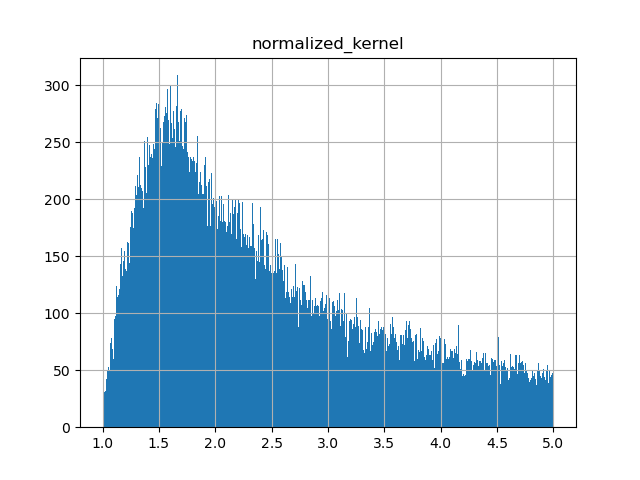
\includegraphics[width=\linewidth]{figures/normalized_kernel_histogram_lt5.png}
  \caption{Distribution of normalized execution times for all benchmark models
  with the template schedule using parameter values as shown in Table \ref{tab:schedparams}}. 
  \label{Fig:ExecTimeDistribution}
\end{figure}

We evaluated all the schedules in this space on several real world models and observed that 
there is huge variation in performance with different parameter values. 
Figure \ref{Fig:ExecTimeDistribution} shows the distribution of normalized execution times
for some real-world models with different parameter values for the template schedule (inference
times normalized w.r.t fastest time for that model).
As can be seen very few schedules perform close to the best while a vast majority of
schedules perform poorly.

Exhaustive exploration over this bounded space ($5184$ schedules) is still very expensive, taking
anywhere between thirty minutes to a few hours to explore the entire space for a given model. 
%Exploring the space for every model is infeasible.
%\TODO{comment on online vs offline exploration? Set a goal for the heuristic?}

\subsection{Pruning the search space}
%Exploring the schedule space extensively even for a reasonable set of parameter values is very expensive.
 
%Performing this extensive search for every model being compiled is infeasible in practise. 
A careful analysis of the search space reveals that certain schedules are not likely to 
perform well as they either do not exploit the parallelism available in the model or do not take advantage of the hardware features.
We use a combination of 3 strategies to further prune the search space.
Algorithm \ref{alg:heuristic} presents our final heuristic to find a good schedule.
%need a better mechanism to guide the search for a good schedule.

\subsubsection*{Insufficient parallelism}
 Some configurations do not expose sufficient parallelism, we prune these out.
  For example when the batch size is small, it does not make sense to have a many rows
  per thread block or to partition the trees across a few threads. 
  We therefore limit the combinations used based on batch size (see lines 3---8).
\subsubsection*{Utilizing shared memory}
  Shared memory is a critical resource on GPUs and it helps to only bring objects that would be reused into it. 
  We observe that tree nodes have limited reuse and the one time cost of loading trees is not sufficiently amortized when the whole tree is not accessed during inference. 
  On the other hand caching rows 
  %when possible (i.e., when the number of features is small enough to fit in shared memory)
  almost always improves performance. Further when the inputs have many features, it may not be possible to cache all rows.
  In this scenario it helps to retain a few rows in memory, and pick schedules similar to the small batch size case (lines 15,3---5).

  %trees across more threads even at larger batch sizes. This is because processing fewer rows at a time 
  %allows us to keep them in shared memory.
  % We empirically find that the threshold for when 
  % we should start partitioning the trees across more threads is when the number of features
  % is greater than 100. 
  \subsubsection*{Orthogonal parameters} We find that some parameters like reduction type are orthogonal to the rest. 
  We therefore break the exploration into two phases, first we pick the best schedules without reduction
  optimizations and then evaluate reduction options on the best schedules.
  %We find that when a model prefers schedules with shared reduction, the same schedules 
  %without shared reduction are among the best performing schedules without shared reduction.
  % We therefore are able to separate the evaluation of shared reduction by collecting the 
  % best schedules without shared reduction and only evaluating shared reduction on them. 
  Evaluating the top 3 schedules for reduction is sufficient in practice.  

\begin{comment}
\Treebeard{} uses these observations to narrow down the set of schedules to explore. 
The pseudo-code for the heuristic is shown in Algorithm \ref{alg:heuristic}.
The algorithm first computes a subset of thread block configurations in the function 
\op{TBConfigs}. A set of schedules based on these thread block configurations 
is then computed (\op{schedules}). 
\end{comment}

\noindent
\Treebeard{} performs an exhaustive search over the pruned schedules from Algorithm~\ref{alg:heuristic} to find the best schedule.
The model is compiled with each of these schedules and evaluated on a few input batches. 
%The three best performing schedules 
%are collected and shared reduction is enabled on them and the resulting schedules evaluated.
The best schedule among all the evaluated schedules is selected as the schedule to use.
We report that this heuristic is able to find schedules that are close to the best schedules
while improving the search time by two orders of magnitude (see Section \ref{sec:results}).

\begin{algorithm}
  \caption{Heuristic to find a good schedule}
  \label{alg:heuristic}
  \small{
  \begin{algorithmic}[1]
  \Procedure{TBConfigs}{$N_{batch}$, $N_f$}
    \State $T_{batch} \gets 2048,\; T_f \gets 128$
    \If {$N_{batch} \leq T_{batch}$ \textbf{or} $N_{f} > T_{f}$}
      \State $rowsPerBlock \gets \{8, 32\}$
      \State $treeThreads \gets \{20, 50\}$
    \Else
      \State $rowsPerBlock \gets \{32, 64\}$
      \State $treeThreads \gets \{2, 10\}$
    \EndIf
    \State \Return $rowsPerBlock, treeThreads$
  \EndProcedure
  \\
  \State $bestSchedules \gets shMemSchedules \gets \emptyset$
  \State $rowsPerTB, treeThds \gets TBConfigs(N_{batch}, N_f)$
  \State $cacheRows \gets \text{True},\; cacheTrees \gets \text{False}$
  \State $interleave \gets \{1, 2, 4\}$
  % \State $reps \gets \{array, sparse, reorg\}$
  \State $schedules \gets (rowsPerTB, treeThds, cacheRows,$ \\
                          \hspace{2cm}$cacheTrees, interleave)$
                          %\hspace{2cm}$$
  \For{$(sched, rep) \in schedules \times \{array, sparse, reorg\}$}
    \State $time \gets EvaluateSchedule(sched, rep)$
    \State $bestSchedules.insert(time, sched, rep)$
  \EndFor
  \State 
  \For{$sched, rep \in Top3(bestSchedules)$}
    \State $EnableSharedReduction(sched)$
    \State $time \gets EvaluateSchedule(sched, rep)$
    \State $shMemSchedules.insert(time, sched, rep)$
  \EndFor
  \State \Return $min(shMemSchedules \cup bestSchedules)$
  \end{algorithmic} 
  }
\end{algorithm}
\section{Experimental Evaluation}
\label{sec:results}

We evaluate \Treebeard{} on several machines. The first machine has an AMD Ryzen 9 7950X 16-Core processor,
128 GB of RAM, an NVIDIA RTX 4060 GPU with 8 GB of RAM and runs Ubuntu 22.04.2 LTS with CUDA 11.5. The 
second has an Intel Core i9-11900K (Rocket Lake) processor with 8 physical cores, 128 GB of RAM, an 
NVIDIA T400 with 2GB of RAM and runs Ubuntu 20.04.3 LTS with CUDA 11.8. We also evaluate \Treebeard{} on 
an AMD MI210 GPU. To establish the efficacy of \Treebeard{}, we compare it with NVIDIA RAPIDs v23.10,
Tahoe, and XGBoost v1.7.6. We use the same benchmark models as in the \TreebeardOLD{} paper\cite{Treebeard}.
We also evaluate \Treebeard{} on a set of randomly generated models.

\subsection{Performance on Random Models}
\begin{itemize}
  \item Generated a set of over 700 random models with varying depths (6, 7, 8), number of trees (100 - 1000 in steps of 100), 
  and number of features (powers of 2 between 8 to 1024 inclusive).
  \item Compared the kernel time speedup of \Treebeard{} vs RAPIDs on the RTX 4060. The schedule used was the one picked by the auto-tuner. 
  \item Speedups range between 1.5$\times$ and 8$\times$. \Treebeard{} outperforms RAPIDs on all models and batch sizes tested.
  \item Figure \ref{fig:randomModels4060} shows the speedup for models of depth 8 and batch size 512 and depth 6 and batch size 4096.
  Trends for other batch sizes and depths are similar.
\end{itemize}

\begin{figure*}[ht]
  \centering
  \begin{subfigure}[b]{.45\textwidth}
    \subcaptionbox*{}{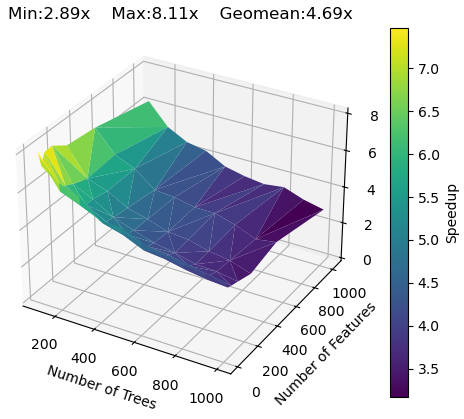
\includegraphics[width=\textwidth]{figures/RandomModels/kernel_speedup_b512_depth8.png}}
    \caption{Batch size 512, depth 8}
  \end{subfigure}
  \begin{subfigure}[b]{.45\textwidth}
    \subcaptionbox*{}{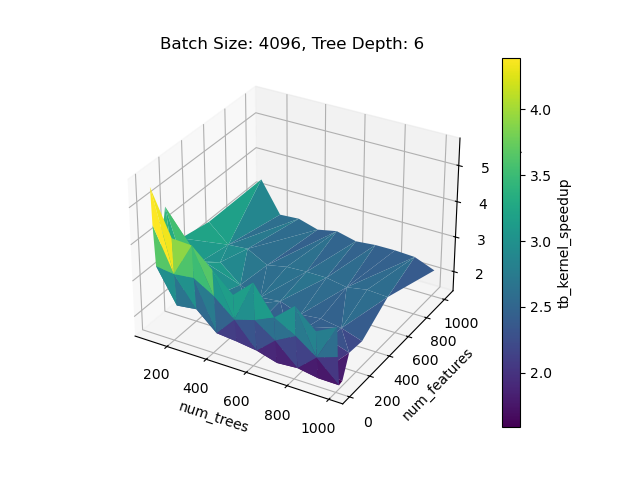
\includegraphics[width=\textwidth]{figures/RandomModels/kernel_speedup_b4096_depth6.png}}
    \caption{Batch size 4096, depth 6}
  \end{subfigure}
  \hfill
  \caption{\label{fig:randomModels4060}\Treebeard{} vs RAPIDs Kernel Time Speedup on NVIDIA RTX 4060 for several randomly generated models.}
\end{figure*}

\subsection{Comparison with RAPIDs, Tahoe and XGBoost}
\begin{itemize}
  \item Measured both the kernel time and total time (time including transferring data to the 
  GPU and results back) for RAPIDs and \Treebeard{}.
  \item Tahoe only allows us to measure the kernel time since it is written as an executable 
  that performs inference repeatedly on the same data that is transferred to the GPU once.
  \item Tahoe does not support multiclass models. We just ran the multiclass models (\op{covtype} and \op{letters})
  as regression models for the comparison. Tahoe also gives wrong results (as reported by its own tests) for 
  \op{letters} and \op{year}. In these cases, we pick the time of the fastest variant that gives the correct results.
  \item Compared the kernel time and total time speedup of \Treebeard{} vs RAPIDs on the RTX 4060 and T400.
  \item Compared the total time speedup of \Treebeard{} vs XGBoost on the RTX 4060.
  \item The schedule used was the one picked by the auto-tuner.
  \item \Treebeard{} outperforms RAPIDs at all batch sizes as shown in Figure \ref{Fig:TBvsRAPIDsTahoe_4060_Speedup}. 
  \item \Treebeard{} outperforms Tahoe on all models and batch sizes tested. Individual benchmark speedups range between 1.1$\times$ and 16$\times$.
  \item \Treebeard{} is faster than XGBoost by more than an order of magnitude. Results are not shown because the speedups don't fit on the same graph.
  \item Figure \ref{Fig:TBvsRAPIDs_4060_TotalTimeSpeedup} shows that \Treebeard{} offers substantial speedup over RAPIDs even when 
  data needs to be transferred to the GPU and results need to be transferred back.
  \item Figure \ref{Fig:TBvsRAPIDsTahoe_T400_Speedup} shows that these speedups are also observed on the T400 thus showing 
  that \Treebeard{} offers portable performance across different GPUs.
  \item Figure \ref{Fig:KernelTimeIndividualBenchmarks4060} shows that \Treebeard{} outperforms RAPIDs and Tahoe on 
  individual benchmarks on the RTX 4060 at small (1024) and large (8192) batch sizes. These batch sizes 
  require different schedules, but the \Treebeard{} auto-tuning heuristic is able to find them.
  % \item Figure \ref{Fig:TotalTimeIndividualBenchmarks4060} compares the total time of \Treebeard{} vs RAPIDs on individual benchmarks. 
  % It shows that even with the overhead of data transfers, \Treebeard{} offers significant speedup. The graph in Figure \ref{Fig:TotalTimeIndividualBenchmarks4060} 
  % shows the breakup of the total time into kernel time and data transfer time.
\end{itemize}

\begin{figure}[htb]
  \centering
  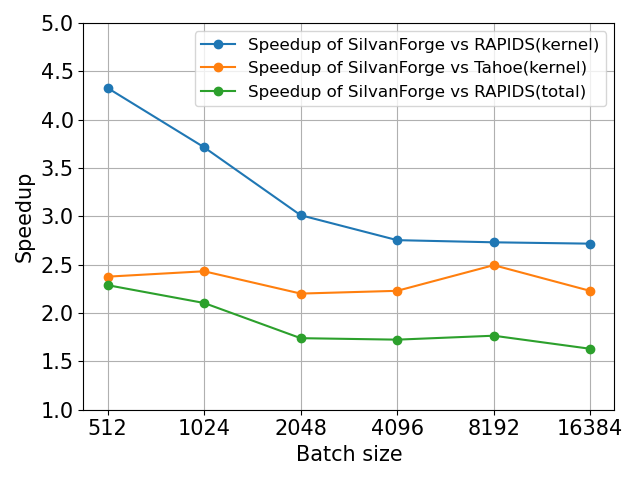
\includegraphics[width=0.75\linewidth]{figures/geomean_speedup_4060_kernel_time_total_time.png}
  \caption{\Treebeard{} vs RAPIDs and Tahoe kernel time and total time speedup on NVIDIA RTX 4060}
  \label{Fig:TBvsRAPIDsTahoe_4060_Speedup}
\end{figure}

% \begin{figure}[htb]
%   \centering
%   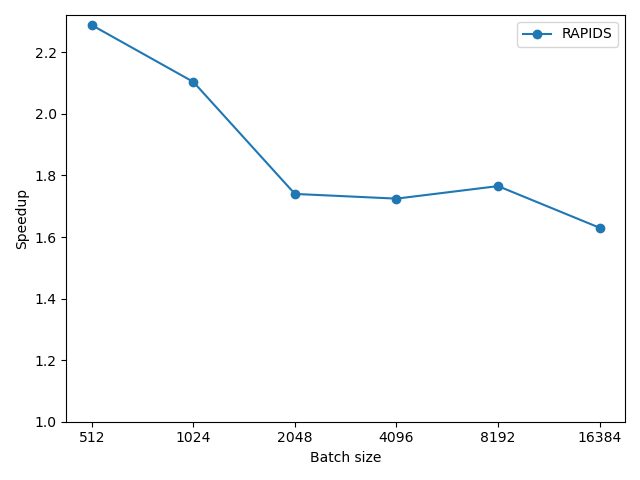
\includegraphics[width=0.75\linewidth]{figures/geomean_speedup_4060_total_time.png}
%   \caption{\Treebeard{} vs RAPIDs Total Time Speedup on NVIDIA RTX 4060.}
%   \label{Fig:TBvsRAPIDs_4060_TotalTimeSpeedup}
% \end{figure}

\begin{figure*}[ht]
  \centering
  \begin{subfigure}[b]{.45\textwidth}
    \subcaptionbox*{}{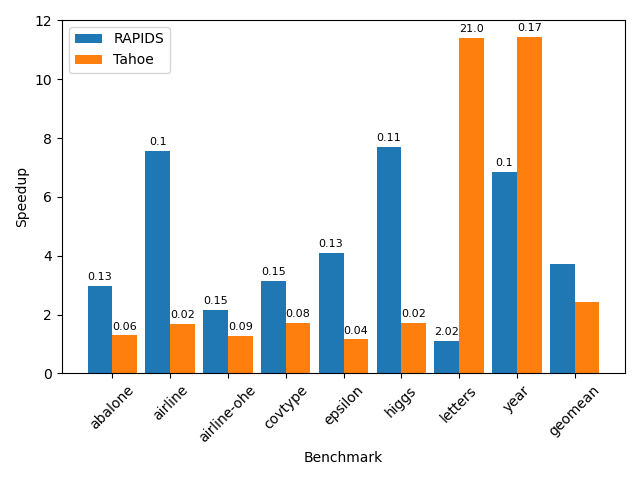
\includegraphics[width=\textwidth]{figures/speedup_bar_graph_1024.png}}
    \caption{Batch size 1024}
  \end{subfigure}
  \begin{subfigure}[b]{.45\textwidth}
    \subcaptionbox*{}{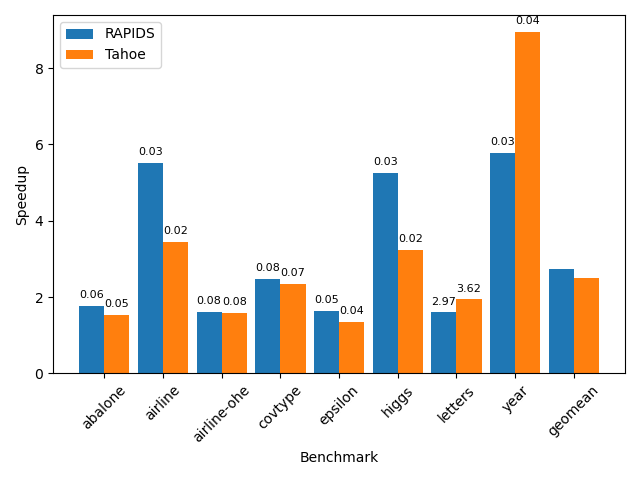
\includegraphics[width=\textwidth]{figures/speedup_bar_graph_8192.png}}
    \caption{Batch size 8192}
  \end{subfigure}
  \hfill
  \caption{\label{Fig:KernelTimeIndividualBenchmarks4060}Kernel time speedup of \Treebeard{} vs RAPIDs on NVIDIA RTX 4060. Numbers on the bars are 
  inference times per sample in $\mu$s for RAPIDs and Tahoe.}
\end{figure*}

\begin{figure}[htb]
  \centering
  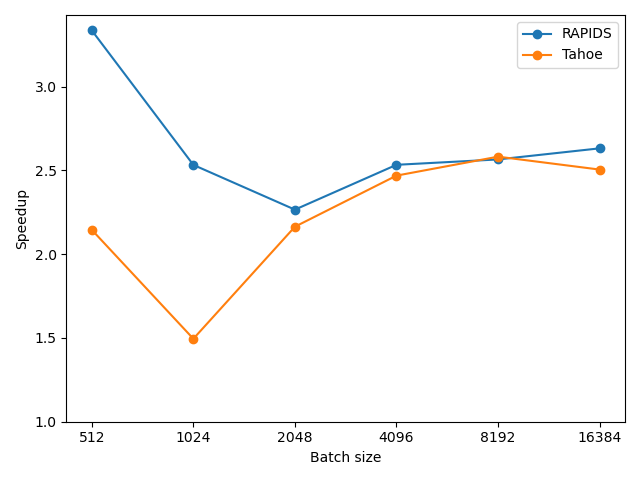
\includegraphics[width=0.75\linewidth]{figures/geomean_speedup_T400_kernel_time.png}
  \caption{\Treebeard{} vs RAPIDs and Tahoe Kernel Time Speedup on NVIDIA T400.}
  \label{Fig:TBvsRAPIDsTahoe_T400_Speedup}
\end{figure}

% \begin{figure*}[ht]
%   \centering
%   \begin{subfigure}[b]{.45\textwidth}
%     \subcaptionbox*{}{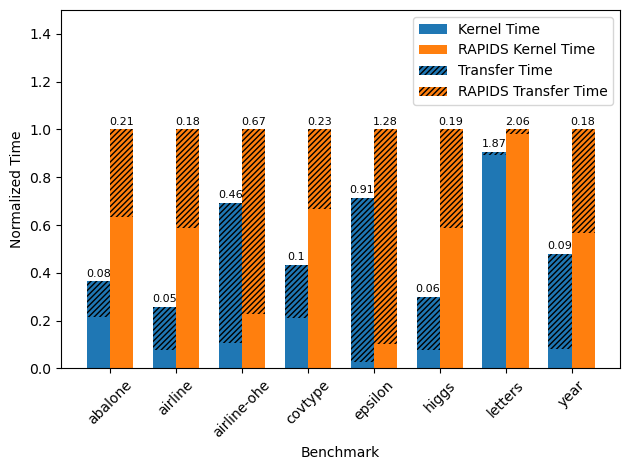
\includegraphics[width=\textwidth]{figures/abs_times_bar_graph_1024.png}}
%     \caption{Batch size 1024.}
%   \end{subfigure}
%   \begin{subfigure}[b]{.45\textwidth}
%     \subcaptionbox*{}{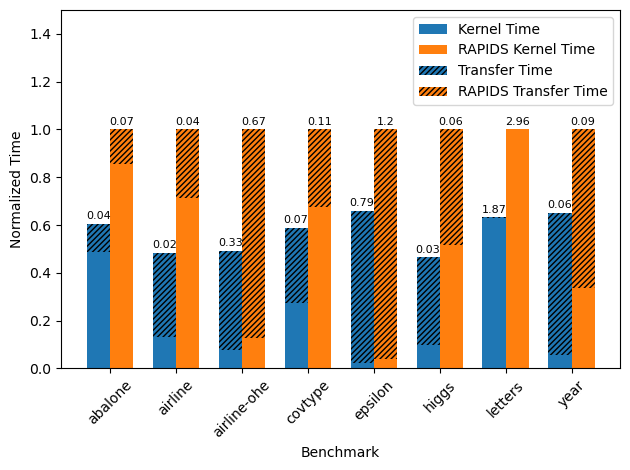
\includegraphics[width=\textwidth]{figures/abs_times_bar_graph_8192.png}}
%     \caption{Batch size 8192.}
%   \end{subfigure}
%   \hfill
%   \caption{\label{Fig:TotalTimeIndividualBenchmarks4060}\Treebeard{} vs RAPIDs total time comparison on NVIDIA RTX 4060. Numbers on the bars are the times 
%   per sample in $\mu$s for \Treebeard{} and RAPIDs. Times for each benchmark are normalized w.r.t the RAPIDs time for that benchmark.}
% \end{figure*}

% \begin{figure}[htb]
%   \centering
%   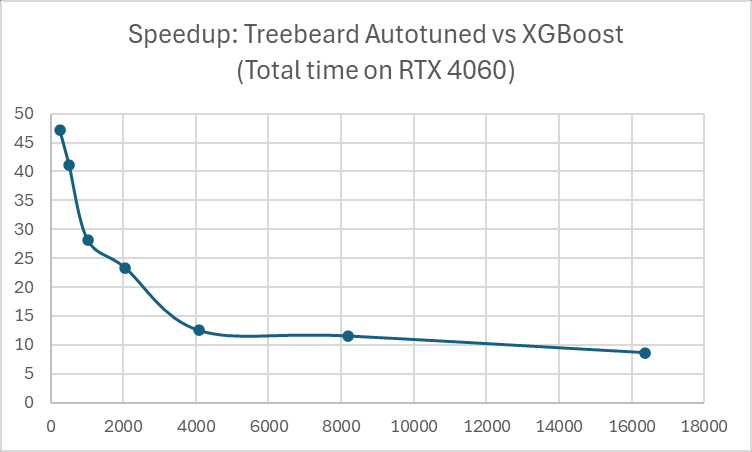
\includegraphics[width=0.75\linewidth]{figures/TBvsXGB_TotalTime.png}
%   \caption{\Treebeard{} vs XGBoost Speedup on RTX 4060.}
%   \label{Fig:TBvsXGBoost_Speedup}
% \end{figure}

\subsection{Autotuning Heuristic}
\begin{figure}[htb]
  \centering
  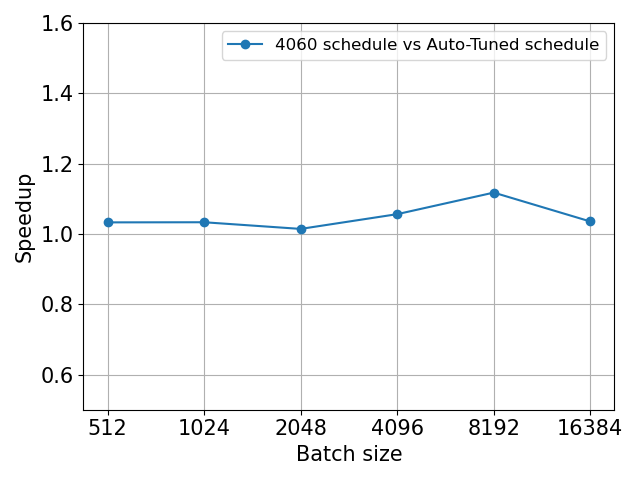
\includegraphics[width=0.75\linewidth]{figures/geomean_speedup_T400_4060_vs_T400.png}
  \caption{Autotuning heuristics speedup vs best 4060 schedule on NVIDIA RTX 4060}
  \label{Fig:AutotuningSpeedupvs4060Sched}
\end{figure}

% \begin{figure}[htb]
%   \centering
%   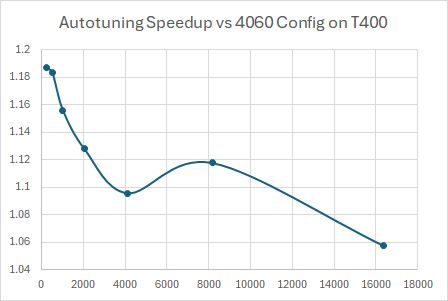
\includegraphics[width=0.75\linewidth]{figures/AutotuningSpeedupvs4060Sched_T400.png}
%   \caption{Autotuning heuristics speedup vs best 4060 schedule on T400.}
%   \label{Fig:AutotuningSpeedupvs4060Sched_T400}
% \end{figure}

\begin{figure}[htb]
  \centering
  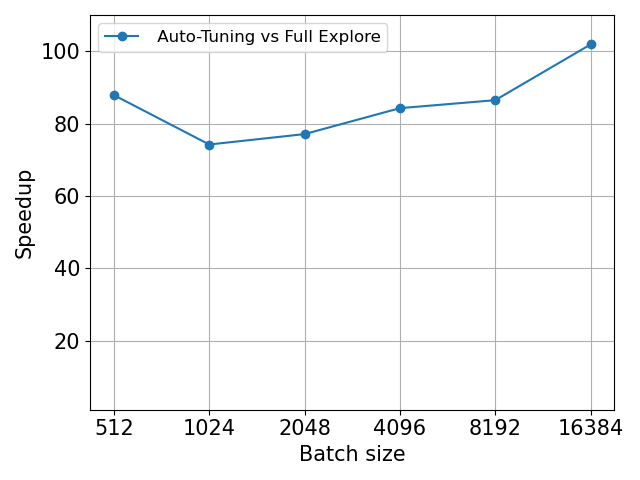
\includegraphics[width=0.75\linewidth]{figures/geomean_speedup_4060_full_exp_vs_at.png}
  \caption{Autotuning heuristic compile time speedup vs full schedule exploration.}
  \label{Fig:HeuristicVsFullExplore_Speedup}
\end{figure}

\begin{itemize}
  \item We compare the schedule found by the schedule exploration heuristic on the RTX 4060 with the best schedule found by
  extensive exploration. Figure \ref{Fig:HeuristicVsFullExplore_Speedup} shows that the heuristic is able to find schedules that are
  very close to the best schedule found by exhaustive exploration.
  \item The speedup of the heuristic schedule vs the best 4060 schedule when run on T400 is shown in Figure \ref{Fig:AutotuningSpeedupvs4060Sched}.
  Geomean speedup ranges from 1.05$\times$ to 1.2$\times$. 
  \item Unsurprisingly, there is some variation in the best schedule for a model even across NVIDIA GPUs.
\end{itemize}

\subsection{AMD GPU}
\begin{figure}[htb]
  \centering
  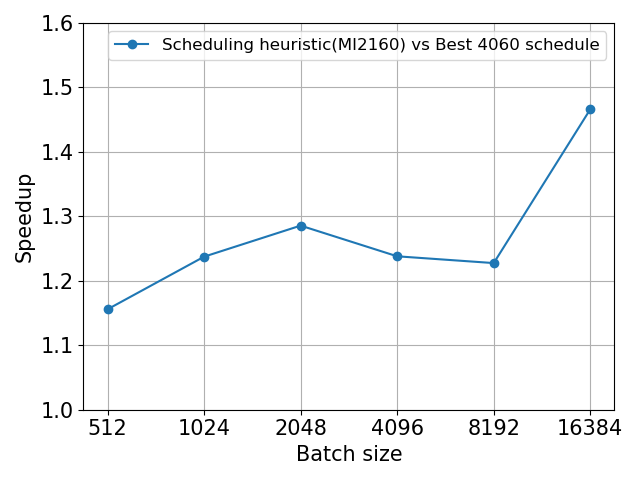
\includegraphics[width=0.75\linewidth]{figures/geomean_speedup_AMDMI2160_4060_vs_MI2160.png}
  \caption{Autotuning heuristics speedup vs best 4060 schedule on MI210.}
  \label{Fig:AMD_MI210_ATHeuristicVs4060Sched_speedup}
\end{figure}

\begin{itemize}
  \item \Treebeard{} is able to compile code to AMD GPUs. We run generated code on an AMD MI210 GPU.
  \item None of the other systems we compare against support running on AMD GPUs. This shows the portability of \Treebeard{}.
  \item The speedup of the heuristic schedule vs the best 4060 schedule when run on the MI210 is shown in Figure \ref{Fig:AMD_MI210_ATHeuristicVs4060Sched_speedup}.
  \item We see that the geomean speedup over all benchmarks is 1.5$\times$ at batch size 16k.
  \item The maximum speedup is 2$\times$ for the \op{letters} benchmark at batch size 16k.
\end{itemize}

\subsection{CPU Improvements}
\begin{itemize}
  \item The ability of \Treebeard{} to parallelize across both trees and rows has a significant impact on CPU performance.
  \item We run experiments on the Intel Core i9-11900K processor to evaluate the impact of parallelizing across trees with small batch sizes. 
  \item At batch size 32, we find that the average speedup over all 8 models is 2.2$\times$ with a max speedup of 5$\times$.
  \item At batch size 64, we find that the average speedup over all 8 models is 1.1$\times$ with a max speedup of 2$\times$. 
  However, we find that 2 of the 8 models show slowdowns in this case. Again, this highlights the need for schedule exploration on CPUs.
  \item For small batch sizes, parallelizing across rows does not work great since there is limited reuse of trees in L1 cache.
  Also, the amount of work per thread is very small leading to high overheads. 
  \item Parallelizing across trees is more effective since there is more reuse in L1 cache and the amount of work per thread is higher.  
\end{itemize}
\section{Related Work}
\label{Sec:Related}
% While several optimization strategies for decision tree based models have been 
% studied in the literature, to the best of our knowledge, no systems that are 
% capable of exploring the full optimization space exist.
This section discusses prior work related to \Treebeard{}.

\emph{Decision Tree Inference Systems:} 
Tahoe~\cite{Tahoe} is a library-based system that picks 
between four predefined strategies to implement decision tree inference on GPUs.
% Also, \Treebeard{} generates code that is specific to 
% a particular model, specializing both the parallelism (by deciding the thread block 
% structure on a per model basis) and the kernel code itself by 
% performing optimizations like tree walk unrolling and interleaving.
% In contrast, Tahoe 
% uses a library-based approach, and cannot generate code tailored to a model 
% like \Treebeard{} does.
RAPIDS FIL\cite{FIL}, the most widely used GPU library for decision tree inference
% implements some heuristics to pick a good configuration for every model, 
% but these techniques are limited and the library uses a single strategy 
% and in-memory representation for all models. 
and XGBoost's\cite{XGBoost} GPU library\cite{XGBGPU} 
use a single strategy and in-memory representation.
In comparison, \Treebeard{} explores a much larger set of implementation options and 
in-memory representations for models and picks the best.
% In contrast, \Treebeard{} is a compiler that can explore a much larger
% optimization space and can generate code that is tailored to a specific model.
As shown in Section \ref{sec:results}, \Treebeard{} outperforms
these systems by a significant margin.
% Finally, all of Tahoe's optimizations are designed to address GPU specific problems. 
% For example, it uses an elaborate and opaque heuristic based on locality sensitive hashing 
% to coalesce accesses to the GPU global memory. We believe that the tree tiling
% infrastructure described in this paper will allow us to deterministically 
% coalesce accesses to GPU global memory.
%As described previously, Hummingbird\cite{Hummingbird} uses tensor operations to perform decision tree inference. 
% While compiling decision tree inference to GPUs presents a distinct set of challenges,
% we believe, we can achieve this while reusing much of \Treebeard{}'s current infrastructure.
% Specifically, we expect that most of the HIR and MIR
% optimizations described in this paper will carry over directly while LIR 
% optimizations and in-memory representations will need to be retargeted.
% This can be the subject of a separate future work.

Some compilers for decision tree ensembles have been proposed in the 
literature \cite{Treelite, Treebeard, Hummingbird}. \TreebeardOLD{} and Treelite
exclusively target CPUs and all their optimizations are designed purely for 
performance on CPUs. 
Treelite\cite{Treelite} is a model compiler that only  
generates \op{if-else} code for each tree in the model. 
\TreebeardOLD{} is the work most closely related to \Treebeard{}. While we 
build on top of \TreebeardOLD{}, \Treebeard{} is a significant enhancement 
over \TreebeardOLD{}. 
Hummingbird\cite{Hummingbird} is a compiler that compiles traditional ML models
to tensor operations, thereby enabling them to be run using tensor-based frameworks like
PyTorch\cite{NEURIPS2019_9015} on CPUs and GPUs. As reported in their paper, Hummingbird's performance
on decision tree models is comparable to that of RAPIDS on GPUs. On CPU, \TreebeardOLD{} 
is faster~\cite{Treebeard}.
% While it can target both CPUs
% and GPUs, its performance has been shown to be lower than that of other frameworks~\cite{Treebeard}.

On CPUs, XGBoost\cite{XGBoost}, LightGBM\cite{LightGBM} and
scikit-learn\cite{Sklearn} are extremely popular.
A recent paper~\cite{PACTVanLunteren} describes an adaptive mechanism 
to pick one of a few predefined parallelization and vectorization strategies.
Other systems that hide dependency stalls by interleaving tree walks\cite{VPred},
implement optimized algorithms for tree inference\cite{QuickScorer, QuickScorer1}
and improve cache performance of decision tree ensembles on CPUs\cite{CacheConscious1, CacheConscious2}
have been proposed in prior work.
Some systems have been proposed to parallelize decision tree training 
on CPUs and GPUs\cite{Jansson2014gpuRFAG, Nasridinov2013DecisionTC}.
However, none of these systems provide portable performance across different target machines.
While the specifics may vary, \Treebeard{} supports retargetable compiler optimizations that 
achieve similar results as techniques in these systems.

\emph{Other Systems and Techniques:} Ren et. al.~\cite{PortableVM} design an
intermediate language and a virtual machine to enable vector execution of decision tree
inference. However, this virtual machine is implemented by 
hand on different target processors.
%This is clearly more expensive than \Treebeard{}'s approach.
% Additionally, even though they perform layout optimizations, their system does
% not perform any model specific optimizations.
Jo et. al.\cite{MilindTreeVectorization} describe code transformations and runtime 
techniques that vectorize tree-based applications but these 
optimizations are not specific to decision trees.
% Both these works vectorize tree walks by performing different tree walks on each
% vector lane. The main issue with this approach is the divergence of tree walks.
% Another issue is that memory accesses are \op{gather}'s rather than vector
% loads. \Treebeard{}'s approach to vectorization solves both these issues. Also,
% these approaches are not precluded by \Treebeard{}'s tiling based vectorization.
% Multiple tiled tree walks can be combined into a single vectorized walk. We
% leave an exploration of this to future work.  FAST\cite{FAST} is a system that
% accelerates tree structured index search on CPUs and GPUs. FAST defines a layout
% for the index tree that enables vectorization of the tree walk. FAST uses a tree
% tiling approach to vectorize tree walks. However, FAST only uses a single
% triangular tile shape. \Treebeard{}'s basic tiling algorithm is a generalization
% of the tiling used in FAST. If given a perfectly balanced tree, the basic tiling
% algorithm would return exactly the tiling used by FAST.  Also, the tree walks in
% FAST are hand coded using intrinsics on the CPU and CUDA on the GPU and
% therefore need repeated effort to implement on each target. 
Inspector-executor systems \cite{TaoOfParallelism,HybridCPUGPU}  
parallelize tree walks but are not a good fit 
for decision tree inference as the individual node predicates are 
simple and the overhead of an inspector-executor system would be prohibitive.

\emph{Code Generation Systems for Other Domains:}
% Several optimizing compilers and code generation techniques have been developed 
% for other domains. 
TVM\cite{TVM}, Tiramisu\cite{Tiramisu}, and Tensor 
Comprehensions\cite{TensorComprehensions} are optimizing compilers 
for DNNs that can target a variety of processors. Similarly, 
Halide\cite{Halide} is a DSL and compiler primarily designed for 
image processing applications. The concept of separating the computation 
from the schedule was effectively utilized by Halide and has since been adopted 
by several other systems~\cite{TVM,Tiramisu,GraphIt}. 
% However, to 
% the best of our knowledge, \Treebeard{} is the first system to design
% a scheduling language for decision tree inference optimization
% and to build a system capable of state-of-the-art performance 
% across different processors.
% {\sc {Cortex}} transforms 
% recursive computations in DNNs to loop based computations and optimizes them.
% However, the model properties {\sc {Cortex}} assumes to optimize
% generated code do not hold in the context of decision tree inference. For example, 
% {\sc {Cortex}} assumes that control flow depends purely on data structure 
% connectivity. This is not the case with decision trees. Control flow is determined 
% by the input value and not by the structure of the tree. This makes the 
% problems addressed by \Treebeard{} very different from the ones handled
% by {\sc {Cortex}}.
Libraries that compose or generate optimized implementations  
for BLAS\cite{BLIS, atlas_sc98, CUTLASS} and signal processing\cite{FFTW, SPIRAL}
have also been developed.
However, \Treebeard{} is the first system that provides state-of-the-art performance
across targets by implementing a scheduling language for decision tree inference.
% BLIS\cite{BLIS} and ATLAS\cite{atlas_sc98}
% are systems to instantiate high performance BLAS routines on multiple 
% target architectures. CUTLASS\cite{CUTLASS} provides building blocks 
% in the form of C++ templates to quickly instantiate high performance 
% BLAS functions on different GPU architectures. SPIRAL\cite{SPIRAL}
% is a domain specific compiler for signal processing applications
% that instantiates high performance routines for linear transformations 
% like FFTs and FIR filters. FFTW\cite{FFTW} is a fast fourier transform 
% compiler that generates high performance FFT routines by customizing 
% the routine based on FFT size and the target machine. 
% However, no such frameworks for decision tree ensembles exist currently.
% \Treebeard{} is a first step in this direction and unlocks several future 
% optimization opportunities.

\emph{Reductions:} CUB\cite{CUB} and Thrust\cite{Thrust} are libraries 
that implement high-performance parallel reductions on GPUs. 
However, it is not possible to fuse these functions with other computations  
as required in \Treebeard{}. Reddy et. al.~\cite{ChandanReduction}
describe language constructs in {\sc {Pencil}}~\cite{Pencil}
to express reductions and to represent and optimize them using the polyhedral 
framework. 
% It is not clear how these techniques can be fused with 
% other computations in arbitrary loop nests as required in \Treebeard{}.
%Additionally, 
Their system does not express the hierarchical nature of 
reductions and also only targets GPUs. Suriana et. al.~\cite{HalideReductions}
extend Halide to add support for factoring reductions in the Halide 
scheduling language and to synthesize reduction operators. De Gonzalo 
et. al.~\cite{TangramReduction} describe a system based on Tangram 
that composes several partial reduction implementations into different 
reduction implementations for GPUs and then searches through these
alternate implementations to find the best ones. In summary, none of 
these systems provide abstractions and a general framework to generate 
and optimize reductions across different target processors as \Treebeard{} does.

%%
%% The next two lines define the bibliography style to be used, and
%% the bibliography file.
\bibliographystyle{ACM-Reference-Format}
\bibliography{refs}

%%
%% If your work has an appendix, this is the place to put it.

\end{document}
\endinput
%%
%% End of file `sample-sigplan.tex'.
